\documentclass[12pt]{report}
%\usepackage{ae} % or {zefonts}
\usepackage[T1]{fontenc}
%\usepackage[utf8]{inputenc}
\usepackage[english]{babel}
\usepackage{makeidx}
\usepackage{amsmath}
\usepackage{amsfonts}
\usepackage{multicol}
\usepackage{float}
\usepackage[small]{caption}
\usepackage{textcomp}

\usepackage{graphicx}
%\usepackage{color}
\usepackage[colorlinks]{hyperref}
%\usepackage{epsfig}
\usepackage[a4paper,margin=2cm]{geometry}

% Get it from CTAN if it is not included in your TEX distribution
%\usepackage{europs}
%\DeclareInputText{128}{\EUR} % ANSI code for euro: �
%   \EURhv   selects EuroSans
%   \EURtm   selects EuroSerif
%   \EURcr   selects EuroMono
%   \EUR    selects one of the three above, depending on the current
%        context
%
%   \EURofc  selects EuroSans Regular independent of context
%        N.B.: This is the only "official" Euro symbol. If you
%           want to conform with the rules of the EU (or
%           whoever), you may only use this symbol.
%
%\usepackage{eurosym}
%\DeclareInputText{128}{\euro} % ANSI code for euro: �

%\usepackage{lscape}
\usepackage{algorithm}% http://ctan.org/pkg/algorithm
\usepackage{algpseudocode}% http://ctan.org/pkg/algorithmicx
\makeatletter
\newlength{\trianglerightwidth}
\settowidth{\trianglerightwidth}{$\triangleright$~}
\algnewcommand{\LineComment}[1]{\Statex \hskip\ALG@thistlm $\triangleright$ #1}
\algnewcommand{\LineCommentCont}[1]{\Statex \hskip\ALG@thistlm%
  \parbox[t]{\dimexpr\linewidth-\ALG@thistlm}{\hangindent=\trianglerightwidth \hangafter=1 \strut$\triangleright$ #1\strut}}
\makeatother

\title{Internship report}
\author{Tamar Huygen \\ tamar@huygen.nl}

\begin{document}
\maketitle

\begin{abstract}
  Participation iGEM 2015 my contribution
\end{abstract}

\chapter{Introduction}

\section*{General Introduction}


-climate change
-our solution
-modelling

\subsection{Sustainability (under construction)}\label{sec:sus}
The main returning theme in this paper is stability. The word stability has 
different meanings in different contexts. In this paper several definitions of 
stability will be discussed. We will start with one that has to do with one of 
the greatest challenges that mankind has to face in this time. The stability of 
our own population, humanity, on this planet.

We might think that we will always be able to live like we were used to on our 
planet, but considering our own population dynamics (see figure 
\ref{fig:owndyn}) and the accompanying demand for energy and food. We can safely 
assume that using resources we cannot replenish, will not be a stable strategy. 
Sooner or later one of the irreplaceable resources will run out. When that 
happens we have to see whether the other resources are able to fill in the gap. 
Until that happens we have to look for more sustainable ways of producing food 
and energy. Resources that cannot run out fast, such as sunlight or geothermal 
energy, have the advantage that they will be a reliable energy source for as 
long as humanity lives on this planet.

In the way we are using the resources of the planet now we also have multiple 
environmental issues. Pollution of the environment may give an (economic) 
advantage on the short term, but polluting strategies are certainly not feasible 
considering longer timespans. 
Then there is also the problem of global warming. Because of the increasing use 
of fossil fuels a lot more CO$_{2}$ is released in the atmosphere and CO$_{2}$ 
levels have been rising. Although there are gasses with higher global warming 
potential, a slight change in the balance of gases in the atmosphere, can have 
an effect on temperature. This slight effect can also have an effect on other 
sources of greenhouse gases, such as release of methane from permafrost tundras 
which are now thawing, enhancing the greenhouse effect. This gas-compositions 
shift and accompanying temperature shift will have major ecological and 
economical consequences on our planet. If we want to slow this process down it 
is of major importance that we reduce the emission of greenhouse gases and 
CO$_2$.

This is were the bio-based economy comes in. More and more entrepreneurs and 
scientists are looking for less polluting ways to produce, where possible also 
with less CO$_2$ emission. They can do this with the help of biotechnological 
advances. In biotechnology, there are also still a lot of challenges. In the 
past food crops have been used to create fuel in a bio-based manner. This caused 
the crop prices to rise in certain areas, which is seen as a great disadvantage. 
We have to find a way to produce in a sustainable manner, without competing with 
food. By choosing a non crop organism, which harvests light and CO$_2$, like 
Synechocystis, we might get a small step closer to reach this goal. 

In an ideal world we would have closed carbon cycles. That which we produce in 
CO$_2$ would also be consumed. In this way we would enhance the stability of the 
environment in which mankind seems to prevail. 

\begin{figure}[!ht]
 \begin{center}  
  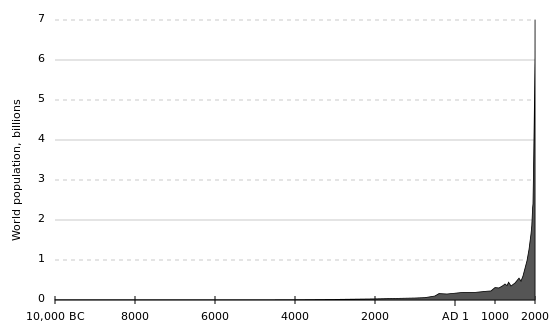
\includegraphics[width=8cm]{human_population_curve.png}
  \caption{Our own population dynamics so far.}
  \label{fig:owndyn}
 \end{center}
\end{figure}

\subsection{Stable bio-production}
Bio-based production usually resolves around an organism producing a compound that is in some way useful to humanity.
An easy way to make a certain organism produce a certain compound in a certain way is to transform the organism with the genes that are needed for the biosynthesis of the product. This means inserting genes
However this is not a very stable form of production. Populations of organisms with

\subsection{Stable consortium}

\subsection{The search for a sustainable solution and synthetic biology}
A lot of different approaches in the search for sustainable production and 
energy harvest have been used. 

\subsection{The team iGEMAmsterdam 2015 Solution}
The iGEM team of 


iGem cyanobacteria, filipe overview literature,
oview project, stability, my contribution
When is something considered stable?
Why a symbiose?
Why Synechocystis?
Why E. Coli?
Why the algorithms?
Why kinetic models?
How does this module fit into the project?

\chapter{Algorithms}

\begin{abstract}
  
\end{abstract}

\section{Introduction}
An important goal in the bio-industry is the production of certain carbon containing compounds. When we let micro-organisms produce these compounds, there is always a stability challenge. Usually it is better in terms of fitness for an organism use all carbon it can for the generation of biomass. So consider an organism which where we have inserted genes which forces the organism to produce a certain compound and transport it out of the cell, so that we may use it. A mutation may yield an organism which does no longer produce the compound. Organisms with this mutation likely have a fitness advantage over organisms without this mutation, because they can use all carbon compounds for generation of biomass and don't leak carbon compound to the environment. This means that soon after the appearance of the mutation the non-productive organisms will take over the entire population and the production stops and has to be re-initiated. We want to address this problem and have created an algorithm which searches for solutions that force an organism to produce a carbon compound, with a much smaller chance of rendering a non-productive population.

\subsection{Models}\label{sec:intro_models}
When studying cells in silico one is always dependent on models. To study metabolism of cells and the connections to the genetic network, flux balance analysis (FBA) has become an important tool. (hier een stukje in appendix over fba?? of hier?)
FBA models consist of a set of differential equations that model the flux of mass through reactions as these reactions are assumed to be in steady state. The models simulate the more or less constant nett flux of mass converted by the reaction.
It is important to note that the base of the model consists simulations of reactions.


Genes play an important role in the models, but only in terms of the influence of the genes on the reactions.
In reality there is a complex interaction between genes, gene regulation, transcription, translation and the reactions.
In our models the genes are only encoded in the influence they eventually have on the flux through the reactions.
The reactions present in the model sometimes have gene associations.
These gene associations list genes, that when present and active, enable the reaction to happen.


If there are multiple genes listed in the gene association they can have an \emph{or} or an \emph{and} relationship.
In figure \ref{fig:genes1}  two reactions are shown with the genes that are listed in the gene associations of these reactions.
For reaction 1 to happen, either gene 1 or gene 2 are has to be active. For reaction 2 both gene 2 and gene 3 are have to be active. So when gene 2 is deactivated or deleted, while gene 1 and gene 3 stay active, reaction 2 is taken out, while reaction 1 is still active. What happens in the model to simulate the inactivity of gene 2 is that the flux of reaction 2 is set to zero.
The models we used were not perfect. Especially the \emph{and} and \emph{or} relationships between the genes cannot be trusted, simply because we don't know these relationships most of the times.
However, as we will see in the next sections, even if these relationships cannot be trusted is still possible to simulate the alternation of a gene in the model.

\begin{figure}[hbtp]
  \centering
     \input{genes1.pdftex_t}
      \caption{Schematic representation of two reactions in the model with their associated genes.}
  \label{fig:genes1}
\end{figure}



\subsection{Stable compound generator}
The goal of the stable compound generator is to find genes which can be deleted in order to create an organism which has to produce a certain carbon compound. Consider the reaction scheme in figure \ref{fig:reaction-overview1}. Our goal is to produce compound B. Our initial plan to achieve this goal is to take out reaction 2. Assume reaction 2 is the only reaction which consumes B. By taking out the reaction we hope the cell will not be able to use B and accumulate and transport it out of the cell.

We have 2 prerequisites to be able to have a stable production of compound B. The first is that reaction 1 is essential for the production of biomass. If cells that don't use reaction 1 are still viable and produce biomass, they will most likely have a fitness advantage over cells that still use reaction 1, because they won't have to produce compound B and can use more carbon for biomass generation. But when cells that take out reaction 1 are non-viable the cells can never take over the population.
The second requirement is that we are able to take out reaction 2 and still yield viable cells, so reaction 2 has to be non-essential for the production of biomass. It is reaction 2 which we want to find. So a first algorithm can look for all reactions that consume B and take all of them out and see if the cells still produce biomass. If so, it returns reaction 2 to us.

\begin{figure}[hbtp]
  \centering
     \input{reaction-overview1.pdftex_t}
      \caption{Scematic overview of a pathway in which carbon compound B is produced, when the net mass flux through reaction 2 becomes zero.}
  \label{fig:reaction-overview1}
\end{figure}

\subsubsection{Combinatorial problems}
The reaction schemes shown in figures \ref{fig:reaction-overview1}, \ref{fig:reaction-overview2} and \ref{fig:reaction-overview3} and are in some way all simplifications. Most reactions have a forward reaction and a reverse reaction. When a reaction is in chemical equilibrium, the forward reaction happens in the same rate as the reverse reaction. This means the net flux of mass through the reaction is zero. Potentially the rate of the reverse reaction can be higher than the rate of the forward reaction. This causes a negative flux through the reaction.

\begin{figure}[hbtp]
  \centering
     \input{reaction-overview2.pdftex_t}
      \caption{Scematic overview of a pathway. The goal is to produce compound B. Normally the net mass flux through reaction 3 is equal to zero. Only when the nett mass flux through reaction 2 becomes zero, the net mass flux through reaction 3 becomes non-zero and compound B is converted to compound D. In order to make the cell produce compound B we have to take out reaction 2 and reaction 3 simultaniously.}
  \label{fig:reaction-overview2}
\end{figure}

Consider figure \ref{fig:reaction-overview2}. Under normal circumstances B is consumed by reaction 2 and reaction 3 is in chemical equilibrium.
Only when reaction 2 is taken out, reaction 3 is used to consume B and the forward flux becomes positive.
In order for the cell to produce B reactions 2 and 3 have to be taken out simultaneously.
An algorithm which searches for reactions that have a mass flux from B to another substance, will only find reaction 2, because initially the flux through reaction 3 is equal to zero. Then after it sets the flux through reaction 2 to zero, the flux through reaction 3 will become positive and the cell would still not produce B. 
To solve this problem the algorithm will have to search for all reactions which are potentially able to consume B. This means all reactions that list compound B as one of its products or as one of its reactants, independent of the mass flux.
An algorithm that would search for these reactions would also list the reaction that initially produces the compound. In figure \ref{fig:reaction-overview2} reaction 1 is such a reaction.
Earlier we assumed reaction 1 is essential for the production of biomass and will yield non-viable cells.
When the algorithm would set the flux of all reactions that list compound B one of its products as well as all reactions that list B as one of its reactants to zero it would also set the flux of reaction 1 to zero. When it then analyzes the model it will find that the cell is not viable anymore. So in order to find the combination of reactions that we have to take out in order for B to be produced (in this case take out reaction 2 and reaction 3, but not reaction 1) we will have to test combinations of reactions.
Another possibility is that there are multiple reactions such as reaction 1 which produce B, and are essential for biomass generation.
This means that we cannot just find reaction 1 and only set the flux through all other compound B involving reactions to zero.
So the algorithm has to list all reactions that potentially consume B, and find a subset of reactions which it can take out such that the cell is still viable and produces B.
In order to find this subset we have to try out all possible subsets. In this scheme the possibilities the algorithm would create the following list of reactions: ${1, 2, 3}$.
Then it will have to create a list of all combinations of these reactions: ${{1},{2},{3},{1,2},{1,3},{2,3}}$ (the list doesn't contain $\emptyset$, nor ${1,2,3}$ because we don't have to try taking out no reactions, because then we wouldn't change the cell and we don't have to try taking out all reactions, because then we will also take out all reactions that produce B and we cannot produce B to begin with).
The algorithm then has to try each of these subsets.
In the example given by figure \ref{fig:reaction-overview2} it is possible to try out all these possibilities within a reasonable amount of time.
In all combinations where reaction 1 is taken out the cells are not viable, so such an algorithm won't return them and in cases where only reaction 2 or reaction 3 is taken out, B won't be produced, so the algorithm also won't return them, but the algorithm will return ${2,3}$ given that reactions 2 and 3 are not essential for cell growth.
However if $n$ is the number of reactions where B is involved in, the amount of possible combinations increases with $2^n$.
This means the algorithm will exponentially become slower with the amount of reactions that are involved.
In the implementation of the algorithm we will define an upper limit of combinations which are tried out before it stops. We will start with combinations in which only a small number of reactions has to be taken out, because this is also the easiest to achieve in vivo.

\subsubsection{Completeness}
\begin{figure}[hbtp]
  \centering
     \input{reaction-overview3.pdftex_t}
      \caption{Scematic overview of a pathway. The goal is to produce compound B. By changing the net mass flux through reaction 4 to zero, compound C might build up, keeping reaction 2 in equilibrium. In this way compound B is also produced. This possible way to produce compound B is overlooked if we only consider reactions that possibly consume compound B.}
  \label{fig:reaction-overview3}
\end{figure}
Now consider the reaction scheme shown in figure \ref{fig:reaction-overview3}.
To produce B we might take out reaction 2, but another possibility might be to take out reaction 4.
When C accumulates the flux through reaction 2 might become 0 and B might also be produced and transported out of the cell.
Our algorithm won't find this possibility, because it only searches for reactions that potentially consume B.
This means our algorithm is not complete and will not return all possible reactions which can be taken out in order to create an organism that produces B.
We have shortly tried to find reactions further down the pathways, but usually this yields almost all reactions of a cell.
This in combination with the earlier described combinatorial problems yields an unusable algorithm.
So for now we accept that the algorithm is not complete and does not guarantee that it finds all possible reactions that can be taken out to produce B.

\subsubsection{From reactions to genes}
Up until now we've only spoken about cells in terms of reactions and our algorithm takes out reactions. In reality it is very hard to influence reactions in cells directly.
More often we try to manipulate reactions that happen in cells through genes.
We can stop reactions for example by taking out genes that encode enzymes which catalyze a reaction.
Since we want to find out what genes we can take out instead of reactions directly, we also would want our algorithm to provide these genes for us.
We can change the algorithm to do this.
The algorithm then has to do the following:
\begin{itemize}
\item List all reactions that potentially consume B
\item List all combinations of reactions that when taken out potentially can make the cell produce B
\item For each combination of reactions just listed, for each reaction in the combination, list the genes associated with the reaction.
\item For each listed gene association list the combination of genes that can be turned of in order to make the reaction no longer happen.
\item For each combination of genes just listed, turn off the genes (this means the algorithm will find each reaction which has the gene in its gene association and determines which of these reactions is taken out when the genes are taken out of this genes and sets the flux through these reactions to 0)
\item Analyze model and check if cell still produces biomass and if compound B is produced.
\item Return successful combinations of genes.
\end{itemize}

\begin{figure}[hbtp]
  \centering
     \input{genes1.pdftex_t}
      \caption{Schematic overview of gene associations without their \emph{and} and \emph{or} relationships.}
  \label{fig:genes2}
\end{figure}

However, like stated in section \ref{sec:intro_models}, we cannot trust the \emph{and} and \emph{or} relationships in the model.
How can we then say anything about which genes we have to alter in order to have the cell create a certain compound?
If we don't know the \emph{and} and \emph{or} relationships, we still have the gene associations, see figure \ref{fig:genes2}.
Assume we want to prevent a certain reaction from happening. Let us call this reaction the primary reaction. Now we assume our algorithm does the following:
\begin{enumerate}
\item Make a list of all genes associated to the primary reaction
\item Make a list of all reactions that have at least one the genes from the list in its gene associations. We will call these reactions secondary reactions.
\item Set the fluxes of all secondary reactions to zero
\item Analyse model
\item Check if cells still grow
\item Check if compound of interest is produced by the cell
\item If cell still grows and produces compound, return set of genes
\end{enumerate}

This algorithm is in two aspects conservative in the solutions it returns.
In reality we are not sure what will happen when only a subset of genes associated to a reaction gets deleted. We want to avoid the risk that a primary reaction still takes place when any of the associated genes is still present. We also don't want to render non-viable cells after we have deleted the genes. A secondary reaction might be essential for cell growth. We want to avoid the risk the algorithm returns a seemingly valid solution, where actually a secondary reaction that is essential for cell growth has been stopped. This is why we assume all secondary reactions are stopped, even though only a subset of the associated genes of these reactions is deleted.

How can we then say anything about which genes we have to alter in order to have the cell create a certain compound?
To solve this problem we try to be conservative when to return a solution. We can let the algorithm list all genes associated with the reactions we want to take out. Then we list all reactions which have one of these genes listed in their gene associations. To take out a certain reaction, we take out all genes associated with it. To simulate this, we take out all reactions which have one of these genes in its gene association. We can see that there are now two contradictory assumptions in play. Consider  In order to take out one reaction we first assume we have to take down all gene associated with it.

\subsection{Auxotrophy sniper}
Auxotrophes are organisms that have an auxotrophy. An auxotrophy is a dependence on a certain compound for a cell to grow. See previous sections.
The general idea is that an auxotroph can be created by knocking out a combination of genes involved in the production of the compound we want to make it dependent on.
The organism should not be able to grow if these genes are knocked out and there is no source for the compound in the extracellular space.
Once again our algorithm searches for such genes. When we found a certain combination of genes we want to test, we deactivate them in the model, and then analyse the model to see if the organism is not able to grow anymore.
When this is the case we create a source in the extracellular space (in this way we simulate adding compound to the medium) and once again analyse the model. Now the organism should be able to grow again. Here follows an overview of how the Auxotrophy Sniper works: 
The algorithm takes a list of compounds of which you want to make a synthesis deficiency in the 
organism of choice. This list can contain for example vitamins or amino acids. For each 
metabolite on the list it does the following:
\begin{itemize}
\item Set flux boundaries of source reaction in the extracellular space (if there is already one 
present) to zero. 
\item Find all primary reactions associated to the compound we want to make the organism 
dependent on. 
\item For each primary reaction, find genes which are associated to the primary reactions. 
\item For each gene find all reactions which have the gene in their gene association 
(secondary reactions). 
\item Make a list of possible combinations of genes which can be knocked out. 
\item Go over the combinations one­by­one, for each gene in a combination turn off primary 
and secondary reactions. 
\item Per combination, do a flux balance analysis and check for biomass formation (growth). 
If it does not form any biomass, a source reaction of the compound is added to the 
model
\item Another flux balance analysis of the model is done and if there is biomass formation 
now, the combination of genes are good candidates. If this combination of genes is 
knocked out the organism will probably become an auxotroph.
\end{itemize}

\section{Methods}
\subsection{Implementation}
\subsubsection{Genes}
Because the models we use are not perfect, the and- and or- relations between the genes cannot be trusted.
We still want the algorithm to return genes. Consider figure !!. Since we cannot trust the \emph{and} and \emph{or} relations, these are left out of the figure. Now if we want to take out reaction 1 we look at all genes associated to it (in this case gene 1 and gene 2). Now we turn off all genes associated to reaction 1. We turn these genes off by finding all reactions which have one of these genes in the gene association. The fluxes of all these reactions are set to 0. So in this case we find gene 1 and gene 2 which are associated with reaction 1. Now we find all reactions which have these genes in its gene association and find reaction 1 (gene 1 and gene 2) and reaction 2 (gene 2). In order to simulate taking out gene 2 we set the fluxes of reaction 1 and reaction 2 to zero. This seems contradictory: we say reaction 1 only stops when all genes associated to it are taken out. While when we just take out gene 2 we assume  

\begin{algorithm}
  \caption{Old (simple) stable compound generator algorithm. We find reactions associated with a certain compound and take a combination of these reactions and switch them of. In reality we cannot switch off reactions, we have to remove genes. This is why this is just a simple version of the algorithm.}\label{alg:scg_old}
  \begin{algorithmic}[1]
    \Procedure{FindReactions}{$compound$, $model$}
        \State $hits \gets \text{\{ \}}$
        \State $r1 \gets [\text{ }]$ 
        \For{$r \in model.reactions$}
        \LineCommentCont{$model.reactions$ gives a list of all reactions in the model. $r$ loops over all these reactions}
            \If{$compound \in r.products \vee compound \in r.reactans$}
            \LineCommentCont{$r.products$ is a list of all products produced by reaction and $r.ractants$ is a list of all reactants of reaction $r$.}
                \State $r1.append(r)$
            \EndIf
        \EndFor
        \If{$length(r1)>1$}
            \State $combinations \gets [comb(r1)]$
            \LineCommentCont{$combinations$ is a list of lists. Each list in combinations contains a combination of reactions that are in r1}
            \State $genes \gets \text{\{ \}}$
            \For{$c \in combinations$}
                \For{$r \in c$}
                    \State $r.flux \gets 0$
                \EndFor
                \State $analyseModel(model)$
                \If{$growth > 0$}
                    \If{$compound \in hits.keys()$}
                        \State $hits[compound].append(c)$
                        \Else{$hits[compound] \gets [c]$}
                    \EndIf
                \EndIf
            \EndFor
        \EndIf
    \EndProcedure
  \end{algorithmic}
\end{algorithm}



\section{Results}
\subsection{Stable compound generator}
het algoritme (een paar relevante algoritmes)
toepassing lijst met genen die mogelijk uit te schakelen zijn
Toepassing van iGem

\section{Discussion}
completeness
sinks
Christine's experiment
opbrengst

\chapter{Kinetic models}

\subsubsection{One-way dependency} \label{sec:un}
Unlimited cell growth is exponentially. The amount of biomass per time for an exponentially growing species can be given by the following different equation:
\begin{equation}
 \frac{da}{dt} = \mu a
\end{equation}
Herein is $a$ the amount of biomass per liter and $\mu$ the growth rate normalized for biomass. One can easily verify that the solution of this differential equation is indeed exponential growth ($a = ce^{\mu t}$). Now from experimental data it has been shown that limited growth on a substrate is a bit different. The normalized growth rate is then dependent on the concentration of substrate. According to the monod equation, the $\mu$ is dependent on $[S]$ in the following way:
\begin{equation}
 \mu = \mu_{max} \frac{[S]}{k_{S}+[S]}
\end{equation}
Herein is $\mu_{max}$ the maximal growth rate (equal to the growth rate at unlimited growth), and $[S]$ the concentration of substrate. $k_S$ is the concentration of $[S]$ at a rate $\frac{1}{2}\mu_{max}$. We also know this equation from enzyme kinetics as the Michaelis-Menten equation. In enzyme kinetics this equation is used to calculate the rates at which enzymes convert products. However the Michaelis-Menten equation is based on theoretical arguments, while Monod is based on experimental findings.
According to Monod, the growth rate saturates as the concentration becomes higher (see figure \ref{fig:monod}).

\begin{figure}[!ht]
 \begin{center}  
     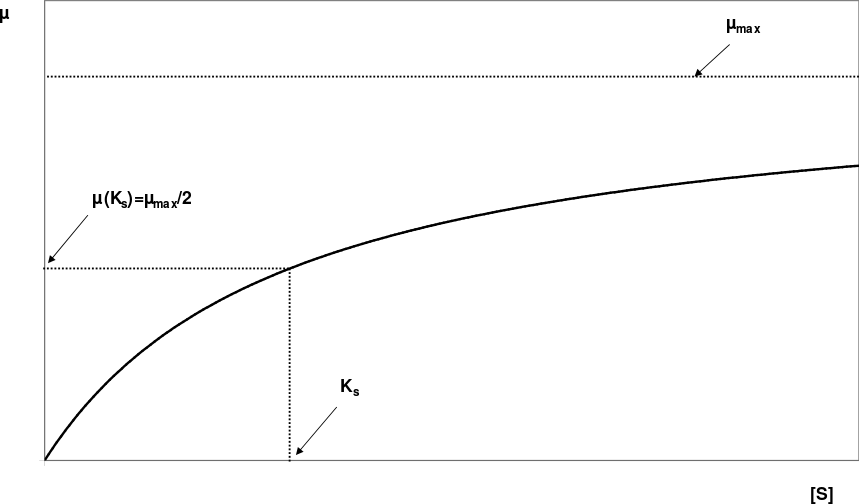
\includegraphics[width=10cm]{Monod_3.png}
     \caption{Limited growth on a substrate according to the Monod equation. $\mu$ is the normalized growth rate in units per hour $\mu_{max}$ is the maximal growth rate and $[S]$ is the substrate concentration. $k_S$ is the concentration at the rate equal to 
     $\frac{1}{2} \mu_{max}$.}
    \label{fig:monod}
    \end{center}
\end{figure}

In our consortium, Escherichia coli grows limited on acetate. So now we know how $\mu$ depends on the concentration of acetate. We now need to model the concentration of acetate. We assume the synthesis of acetate is growth coupled and depends linear on the growth of \textit{Synechocystis}. We also know that the maximal uptake rate of acetate by \textit{E. coli} is dependent $1/y$ herein is $y$ the yield of \textit{E. coli} on acetate in is in milligram Dry Weight \textit{E. coli} per millimole acetate per liter. The uptake of substrate per unit time is also in a a saturable way dependent on the concentration of $S$, exactly the same way the growth speed is dependent on the the concentration of substrate. The synthesis of the substrate is growth coupled  and is dependent on the amount of biomass of \textit{Synechocystis} formed in time. The ch  We now arrived at the following set of differential equations:
\begin{align} \label{eq:ow}
 \frac{d\text{syn}}{dt} &= \mu_{syn}\text{syn} \\
 \frac{d\text{ec}}{dt} &= \mu_{max,ec} \frac{[S]}{k_{s,ec}+[S]} \text{ec} \\
 \frac{d[S]}{dt} &= \frac{1}{y_{s,syn}} \mu_{syn} \text{syn} - \frac{1}{y_{s,ec}} \frac{[S]}{k_{s,ec}+[S]} \text{ec}
\end{align}

Herein is syn the amount of biomass of \textit{Synechocystis} and ec the amount of biomass of E. coli. $y_s$ is the substrate yield of \textit{Synechocystis}. Since in this model the substrate is only formed when \textit{Synechocystis} forms biomass, per amount of biomass formed, there is a constant amount of substrate formed. The yield is usually expressed in gram dry weight mole substrate \emph{used}. In this case we mean gram dry weight mole substrate \emph{formed}. So to find the amount of substrate that is formed per amount of biomass that is formed we simply take $\frac{1}{y,syn}$.

It can be easily seen that such a relationship will not be stable if $\mu_{max,ec}<<\mu_{max,cyn}$. In this case by stability we mean the convergence of the growth rate to the same value.

\subsubsection{Substrate dependent}
In this model, \textit{Synechocystis} is not dependent on E. coli. There are two ways in which \textit{Synechocystis} may be dependent on E. coli we have explored.
Firstly, \textit{E. coli} may produce a substrate \textit{Synechocystis} grows on, as is the case with the auxotrophic \textit{Synechocystis}. Secondly, E. coli may decrease the light intensity in the culture, in this way slowing down the growth of \textit{Synechocystis}. The growth rate of \textit{Synechocystis} can only be limited by one of these two processes and it will always be limited by the process that slows it the most. Either $\mu_{syn}$ is lower than $\mu_{max,syn}$ because there is a photon shortage, but then the amount of substrate available at that growth rate would be enough, or the amount of substrate is limiting, but then the amount of photons available would also be enough for that given growth rate. So actually the growth rate of \textit{Synechocystis} would be 
\begin{equation}\label{eq:min}
 \min(\mu_{max,syn}\frac{[S_{2}]}{k_{s,syn}+[S_2]}, \mu_{max,syn}f(\text{syn},\text{ec}))
\end{equation}
Herein is $f(\text{syn},\text{ec})$ a function which determines the factor of decrease in growth rate because of a photon shortage and it is a function of the amount of biomass per liter of \textit{Synechocystis} as well as that of E. coli.
If we now assume that the amount of substrate E. coli produces is going to be limiting we arrive at the following set of differential equations.

\begin{align} \label{eq:sd}
 \frac{d\text{syn}}{dt} &= \mu_{max,syn} \frac{[S_2]}{k_{s2,syn}+[S_2]} \text{syn} \\
 \frac{d\text{ec}}{dt} &= \mu_{max,ec} \frac{[S_1]}{k_{s1,ec}+[S_1]} \text{ec} \\
 \frac{d[S_1]}{dt} &= \frac{1}{y_{s,syn}} \mu_{max,syn} \frac{[S_2]}{k_{s2,syn}+[S_2]} \text{syn} - \frac{1}{y_{s1,ec}} \frac{[S]}{k_{s1,ec}+[S]} \text{ec} \\
 \frac{d[S_2]}{dt} &=  Q_{p,ec} \text{ec} - \frac{1}{y_{s2,syn}} \frac{[S_2]}{k_{s2,syn}+[S_2]} \text{syn}
\end{align}
Herein is  $Q_{p,ec}$ the amount of $[S_2]$ formed by E. coli per gram dry weight of E. coli. We assume E. coli doesn't produce in a growth coupled way, but has a constant production per amount of biomass.

\begin{align} \label{eq:sd2}
 \frac{d\text{syn}}{dt} &= \mu_{max,syn} \frac{[S_2]}{k_{s2,syn}+[S_2]} \text{syn} \\
 \frac{d\text{ec}}{dt} &= \mu_{max,ec} \frac{[S_1]}{k_{s1,ec}+[S_1]} \text{ec} \\
 \frac{d[S_1]}{dt} &= \frac{1}{y_{s,syn}} \frac{d\text{syn}}{dt} - \frac{1}{y_{s1,ec}} \frac{d\text{ec}}{dt} \\
 \frac{d[S_2]}{dt} &=  Q_{p,ec} \text{ec} - \frac{1}{y_{s2,syn}} \frac{d\text{syn}}{dt}
\end{align}

here
\subsubsection{Light limited growth}
Like stated in section \ref{sec:un}, it is also possible for the photoautotroph to grow light limited instead of substrate limited. As the cell density of both organism increases, the available light for the photoautotroph decreases. In equation \ref{eq:min} it is already suggested that this light dependency might be a function which is dependent on the biomass of \textit{E. coli} and the biomass of \textit{Synechocystis}. But let's first take a look at light dependent growth.
According to literature \cite{franco2006model}, the $\mu$ if a photoautotroph is dependent on the light intensity in the following way:
\begin{equation}
 \mu(I) = \mu_{max,syn}\frac{I}{K_{s,syn}+I+\frac{I^{2}}{K_{i}}}
\end{equation}
Herein is $\mu(I)$ the specific growth rate on light, $\mu_{max,syn}$ the maximal specific growth rate of \textit{Synechocystis}, $I$ the light intensity, $k_{s,syn}$ is the saturation constant on light and $K_{i}$ is an inhibitory constant.
Now the light intensity is not only dependent on the cell density of the photoautotroph and the chemoheterotroph, but it is also dependent on the place in the reactor. However, to not further complicate the model we made a simplification, by assuming the light intensity is linear dependent on the biomass concentration of \textit{Synechocystis} and \textit{E. coli} in the following way:
\begin{equation} \label{eq:I}
 I(\text{syn}, \text{ec}) = \max(I_{max}-sh_{s}\cdot\text{syn}-sh_{e}\cdot\text{ec},0)
\end{equation}
Herein are $sh_{s}$ and $sh_{e}$ 'shading coefficients' for \textit{Synechocystis} and \textit{E. coli} respectively.
In this way the light intensity linear decreases with the amount of biomass of \textit{E. coli} and \textit{Synechocystis}, but it can never be lower than zero.
We then arrive at the following set of differential equations:
\begin{align}
 \frac{d\text{syn}}{dt} &= \mu_{syn} \text{syn} \\
 \frac{d\text{ec}}{dt} &= \mu_{ec} \text{ec} \\
 \frac{d[S]}{dt} &= \frac{1}{y_{s,syn}} \mu_{syn} \text{syn} - \frac{1}{y_{s1,ec}} \mu_{ec} \text{ec} \\
\end{align}
with:
\begin{align}
 \mu_{syn} &= \mu_{max,syn} \frac{I}{I+k_{s,syn}+\frac{I^2}{k_{i}}}\\
 \mu_{ec} &= \mu_{max,ec} \frac{[S]}{[S]+k_{s,ec}}
 \end{align}
With $I$ the light intensity, dependent on the biomass or \textit{E. coli} an \textit{Synechocystis} as given in equation \ref{eq:I}.



\subsection{Turbidostat}\label{sec:turb}
If we want to model the consortium in a turbidostat, we have to account for the fact that both \textit{Synechocystis} and E. coli are increasing the OD as they grow. This means that the dilution rate is dependent on the biomass of \textit{Synechocystis} as well as that of E. coli.
For simplicity we make the assumption that there is a constant flow through the system, instead of only diluting when the threshold is reached.  To understand this we first look at the case of a single strain, called $b$. In a chemostat the growth rate of the organism would become equal to the dilution rate. In a turbidostat however, an organism can grow at its maximal growth rate, but the amount of biomass must still become constant. This means the following:
\begin{equation}
 \frac{db}{dt} = \mu \cdot b - D \cdot b = 0
\end{equation}
Where $b$ is the amount of biomass of the strain $b$, mu is the growth rate and $D$ the dilution rate.\\
In a chemostat it would mean that $D<\mu_{max}$ is a chosen dilution rate and that $\mu$ becomes equal to $D$ due to substrate limitation. In a turbidostat however, $D$ becomes equal to $\mu_{max}$, because the species in not growing limited.\\
In the case where there are two strains, strain $a$ and $b$, that share a turbidostat, the differential equations that then describe the system looks like the following:
\begin{align}
 \frac{da}{dt} &= f(a,b,t) - Da\\
 \frac{db}{dt} &= g(a,b,t) - Db
\end{align}
Herein are $f$ and $g$ functions that describe the growth of the organisms $a$ and $b$ respectively. $D$ is again the dilution rate. Now in a shared turbidostat it holds that $a+b=k$, where $k$ is a constant amount of biomass. Then the following holds:
\begin{alignat}{3}
 & a+b &= k \\
 &\implies \frac{da}{dt} + \frac{db}{dt} &= 0\\
 &\implies f - Da + g - Db & = 0\\
 &\implies Da + Db &= g + f \\
 &\implies D &= \frac{g + f}{a+b}
\end{alignat}
For the turbidostat we then arrive at the following set of differential equations:
\begin{align} \label{eq:turb}
 \frac{d\text{syn}}{dt} &= \mu_{syn}\text{syn} - D\text{syn}\\
 \frac{d\text{ec}}{dt} &= \mu_{ec}\text{ec} - D\text{ec} \\
 \frac{d[S_1]}{dt} &= \frac{1}{y_{syn/S1}} \mu_{syn} \text{syn} - \frac{1}{y_{ec/S1}} \mu_{ec} \text{ec} -D[S_1]\\
 \frac{d[S_2]}{dt} &=  Qp_{S2/ec}\text{ec} - \frac{1}{y_{syn/S2}} \mu_{syn} \text{syn} -D[S_2]
\end{align}
where
\begin{align}
 D &= \frac{\mu_{syn} + \mu_{ec}}{\text{syn}+\text{ec}}\\
 \mu_{syn} &= \mu_{max,syn} \frac{[S_2]}{k_{s2,syn}+[S_{2}]}\\
 \mu_{ec} &= \mu_{max,ec} \frac{S_1}{k_{s1,ec}+[S_1]} \label{eq:turbend}
\end{align}



\section{Results}
\subsection{Batch}
\subsubsection{One-way dependency}
First we simulated the one-way dependent model as depicted by equations \ref{eq:ow}. 
To find out whether the system is robust with respect to the initial conditions we did some simulations. Our expectations were that the biomass ratio of the photoautotroph and the chemoheterotroph in this model would converge irrespective to the initial conditions.
To find out whether the biomass ratio of this system converges, we did some simulations. To be able to make simulations with the models, we have to estimate and measure the parameters.
We tried to measure all parameters as accurate as possible. In table \ref{tab:ol} the measured parameters are given.


\begin{table}[!ht]
 \begin{center}  
  \begin{tabular}{|l|l|}
   \hline
   $\mu_{max,syn}$ ($\text{h}^{-1}$) & 0.075 \\ \hline
   $\mu_{max,ec}$ ($\text{h}^{-1}$) & 0.08 \\ \hline
   $k_{s,ec}$ ($\text{mM}$) & 0.02 \\ \hline
   $y_{\frac{s}{syn}}$ ($\text{mmol}\cdot\text{gDW}^{-1}$) & 0.40 \\ \hline
   $y_{\frac{ec}{s}}$ ($\text{gDW}\cdot\text{mmol}^{-1}$) & 0.031 \\
   \hline   
  \end{tabular}
  \caption{Measured parameters for the one-way dependency model. It can be seen that $\mu_{max,ec} < \mu_{max,syn}$. This is highly unlikely the correct value for $\mu{max,ec}$}
  \label{tab:ol}
 \end{center}
\end{table}

It can be seen from this table, that $\mu_{max,ec} < \mu_{max,syn}$. It is very unlikely that this is correct. It might be caused by experimental Since $\mu$ of \textit{Synechocystis} higher than the $\mu_{max}$ of \textit{E. coli} and given that the growth of \textit{Synechocystis} is independent, we can already expect this model with these parameter to be unstable. \textit{Synechocystis} will keep growing faster than \textit{E. coli}, because the growth rate of \textit{Synechocystis} has a constant value that is higher than the maximal growth rate \textit{E. coli} will ever achieve. If we simulate the model with these parameters find the biomass ratio given in figure \ref{fig:false}. It can be seen that the ratio of biomass does not seem to converge. A more clear image can be seen if we look at the $mu$'s of \textit{E. coli} and \textit{Synechocystis} in figure \ref{fig:false2}.

\begin{figure}[!ht]
 \begin{center}  
     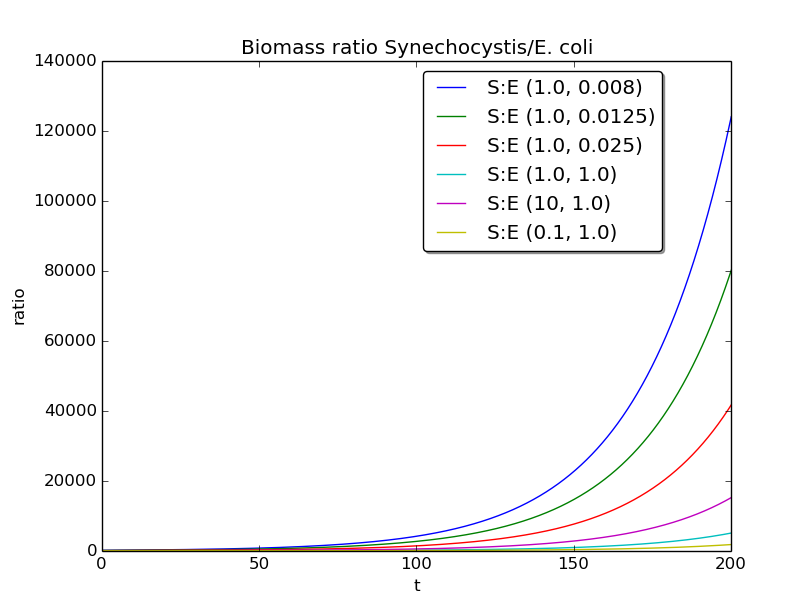
\includegraphics[width=10cm]{independent_flask_ratios_low_mumaxe.png}
     \caption{Boiomass ratio's of \textit{Synechocystis}/\textit{E. coli} in time. They seem to diverge, dependent on the initial conditions. This seems logical, since the growth rate of \textit{E. coli} will never become as high as that of \textit{Synechocystis}. In the legend the initial ratio of \textit{Synechocystis} biomass : \textit{E. coli} biomass is given. The model is given by equations \ref{eq:ow}. Parameters are given by table \ref{tab:ol}}
    \label{fig:false}
    \end{center}
\end{figure}


\begin{figure}[!ht]
 \begin{center}  
     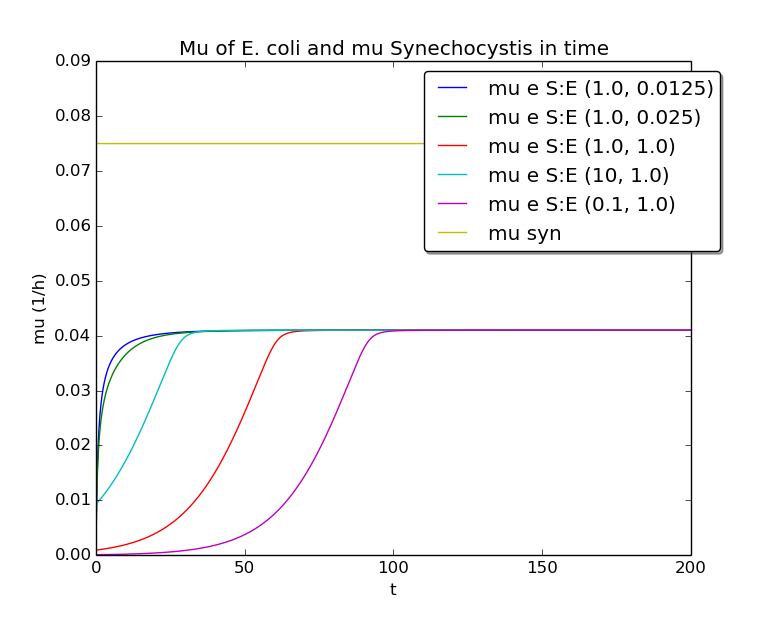
\includegraphics[width=10cm]{independent_flask_mus_low_mumaxe.png}
     \caption{$\mu_{syn}$ and $\mu_{ec}$ under several different initial conditions (shown in legend in $gDW\cdot \text{l}^{-1}$). $\mu_{ec}$ converges to $\mu_{max,ec}$, while $\mu_{syn}$ stays constant at the value of $\mu_{max,syn}$. The model is given by equations \ref{eq:ow}. Parameters are given by table \ref{tab:ol}}
    \label{fig:false2}
    \end{center}
\end{figure}

Chemoheterotrophs are usually have a really high growth rate compared to photoautotrophs. Even though the maximal growth rate of \textit{E. coli} on Acetate might be less than the maximal growth rate on glucose, it is very unlikely that the maximal growth rate is less than that of Synechocystis. So, the question remains, will the biomass ratio converge if we change the parameters such that $\mu_{max,ec} > \mu_{max,syn}$?
To test this we have increased $\mu_{max,ec}$ tot 0.08, which is just higher than the growth rate of Synechocystis. In table \ref{tab:oh} the new parameters are shown.

\begin{table}[!ht]
 \begin{center}  
  \begin{tabular}{|l|l|}
   \hline
   $\mu_{max,syn}$ ($\text{h}^{-1}$) & 0.075 \\ \hline
   $\mu_{max,ec}$ ($\text{h}^{-1}$) & 0.08 \\ \hline
   $k_{s,ec}$ ($\text{mM}$) & 0.02 \\ \hline
   $y_{\frac{s}{syn}}$ ($\text{mmol}\cdot\text{gDW}^{-1}$) & 0.40 \\ \hline
   $y_{\frac{ec}{s}}$ ($\text{gDW}\cdot\text{mmol}^{-1}$) & 0.031 \\
   \hline   
  \end{tabular}
  \caption{Measured and estimated parameters for the one-way dependency model. It can be seen that now $\mu_{max,ec} > \mu_{max,syn}$.}
  \label{tab:oh}
 \end{center}
\end{table}

In figure \ref{fig:oneratio}, the biomass ratio over time given several different initial conditions is shown. Now the biomass ratio does seem to converge. However, this ratio is more than ten times higher than what is found in the lab. This might suggest that we still use inaccurately measured parameters. 

\begin{figure}[!ht]
 \begin{center}  
     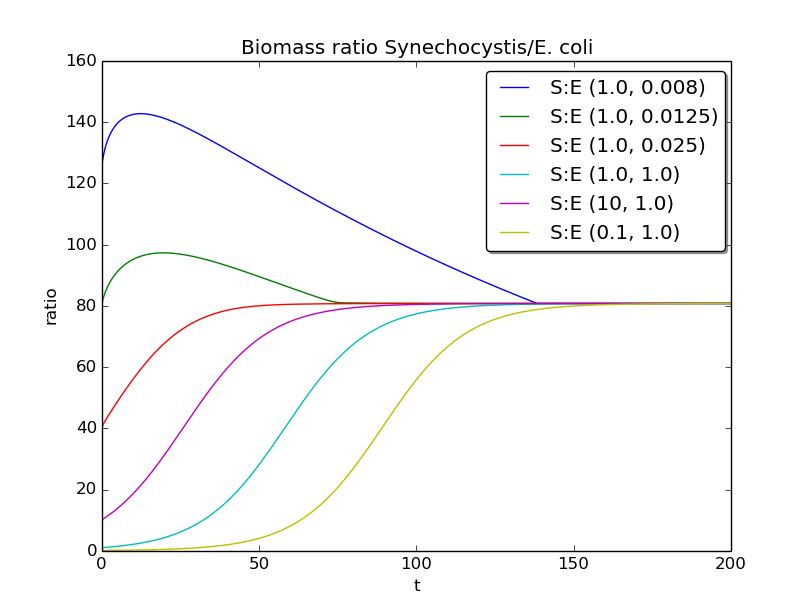
\includegraphics[width=10cm]{independent_flask_ratios.png}
     \caption{The biomass ratio of \textit{Synechocystis} \textit{E. coli} under several different initial conditions (shown in legend in $gDW\cdot \text{l}^{-1}$). The biomass ratio converges to a constant ratio. The model is given by equations \ref{eq:ow}. Parameters are given by table \ref{tab:oh}}
    \label{fig:oneratio}
    \end{center}
\end{figure}

If we look once again at the $\mu$'s over time in figure \ref{fig:onemu} we can see that the $\mu_{ec}$ converges to $\mu_{sys}$. This is quite intuitive, since the growth rate of \textit{E. coli} is limited by the production of substrate, which is dependent on the growth rate of \textit{Synechocystis}. And the biomasses can only converge to a stable ratio, if the growth rates of both species converge to the same value. 
We can conclude that the system now is robust with respect to the initial values.

\begin{figure}[!ht]
 \begin{center}  
     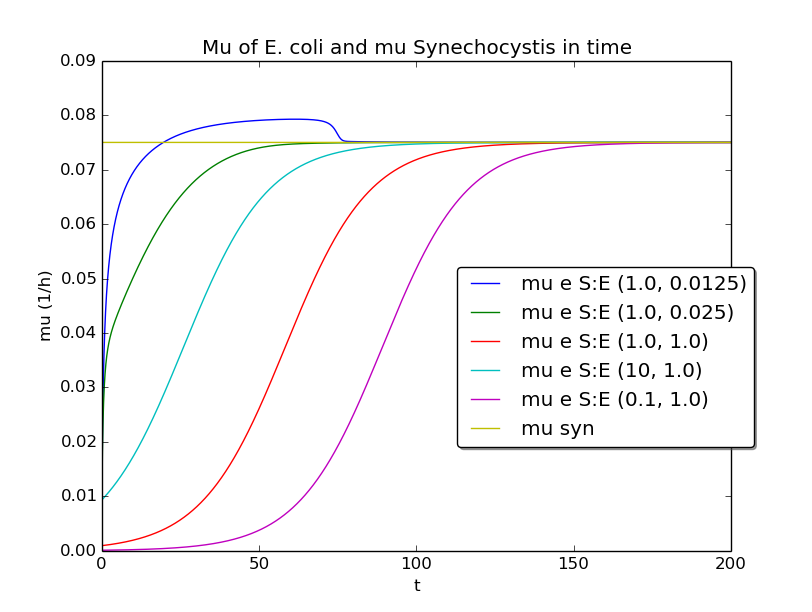
\includegraphics[width=10cm]{independent_flask_mus.png}
     \caption{$\mu_{syn}$ and $\mu_{ec}$ under several different initial conditions (shown in legend in $gDW\cdot \text{l}^{-1}$). The $\mu_{ec}$ converges to $\mu_{syn}=\mu_{max,syn}$. The model is given by equations \ref{eq:ow}. Parameters are given by table \ref{tab:oh}.}
    \label{fig:onemu}
    \end{center}
\end{figure}

\pagebreak
\newpage
\subsubsection{Substrate interdependency}
To simulate the interdependency on substrates, we needed a lot more parameters. For some of the parameters we had no good measurements, so we estimated them. The general behavior stays generally the same under

\begin{table}[!ht]
 \begin{center}  
  \begin{tabular}{|l|l|}
   \hline
   $\mu_{max,syn}$ ($\text{h}^{-1}$) & 0.075 \\ \hline
   $\mu_{max,ec}$ ($\text{h}^{-1}$) & 0.08 \\ \hline
   $k_{s1,ec}$ ($\text{mM}$) & 0.02 \\ \hline
   $k_{s2,syn}$ ($\text{mM}$) & 0.02 \\ \hline
   $y_{\frac{s1}{syn}}$ ($\text{mmol}\cdot\text{gDW}^{-1}$) & 0.40 \\ \hline
   $y_{\frac{ec}{s}}$ ($\text{gDW}\cdot\text{mmol}^{-1}$) & 0.031 \\ \hline
   $y_{\frac{s2}{syn}}$ ($\text{mmol}\cdot\text{gDW}^{-1}$) & 0.1 \\ \hline
   $Q_{p,ec} mmol$ ($\text{mmol}\cdot \text{gDW}^{-1}\cdot\text{h}^{-1}$) & 0.13 \\
   \hline   
  \end{tabular}
  \caption{Measured and estimated parameters for the substrate interdependent model.}
  \label{tab:sdp}
 \end{center}
\end{table}


\begin{figure}[!ht]
 \begin{center}  
     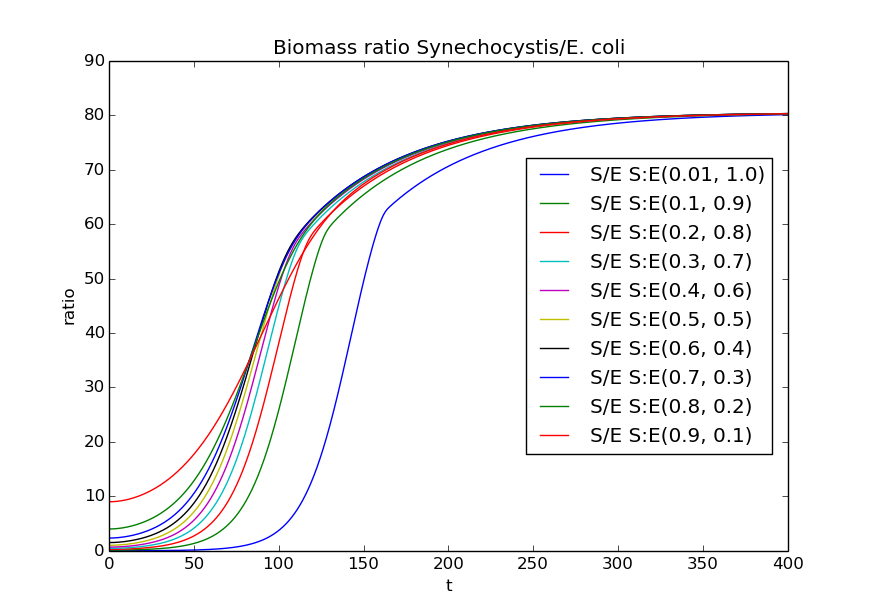
\includegraphics[width=10cm]{ratios_interdependent_1.png}
     \caption{The biomass ratio of \textit{Synechocystis} \textit{E. coli} under several different initial conditions (shown in legend in $gDW\cdot \text{l}^{-1}$). The biomass ratio converges to a constant ratio. The model is given by equations \ref{eq:sd}. Parameters are given by table \ref{tab:sdp}}
    \label{fig:subrat}
    \end{center}
\end{figure}

\begin{figure}[!ht]
 \begin{center}  
     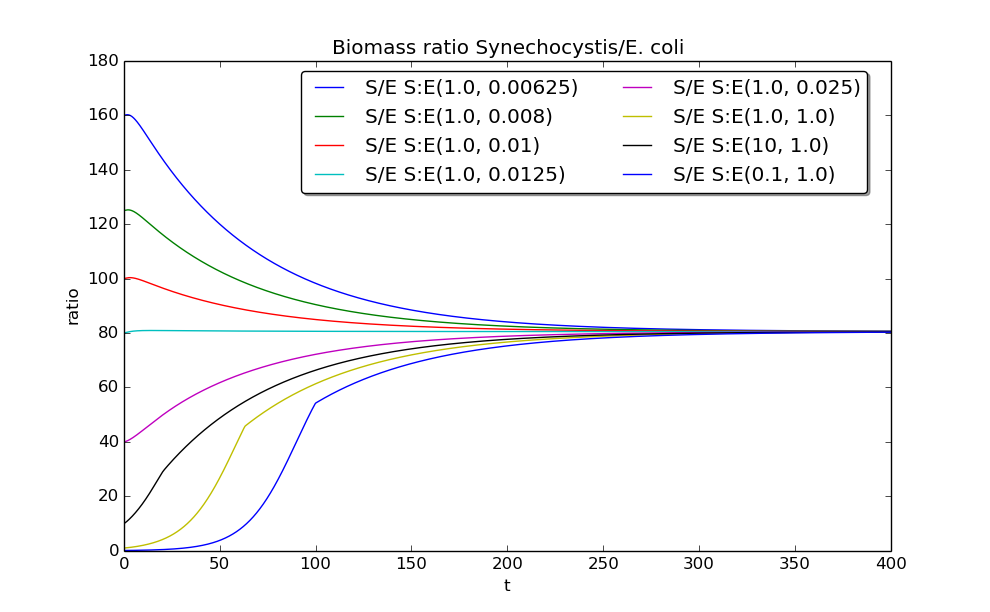
\includegraphics[width=10cm]{ratios_interdependent_2.png}
     \caption{The biomass ratio of \textit{Synechocystis} \textit{E. coli} under several different initial conditions (shown in legend in $gDW\cdot \text{l}^{-1}$). The biomass ratio converges to a constant ratio. The model is given by equations \ref{eq:sd}. Parameters are given by table \ref{tab:sdp}}
    \label{fig:subrat2}
    \end{center}
\end{figure}


\begin{figure}[!ht]
 \begin{center}  
     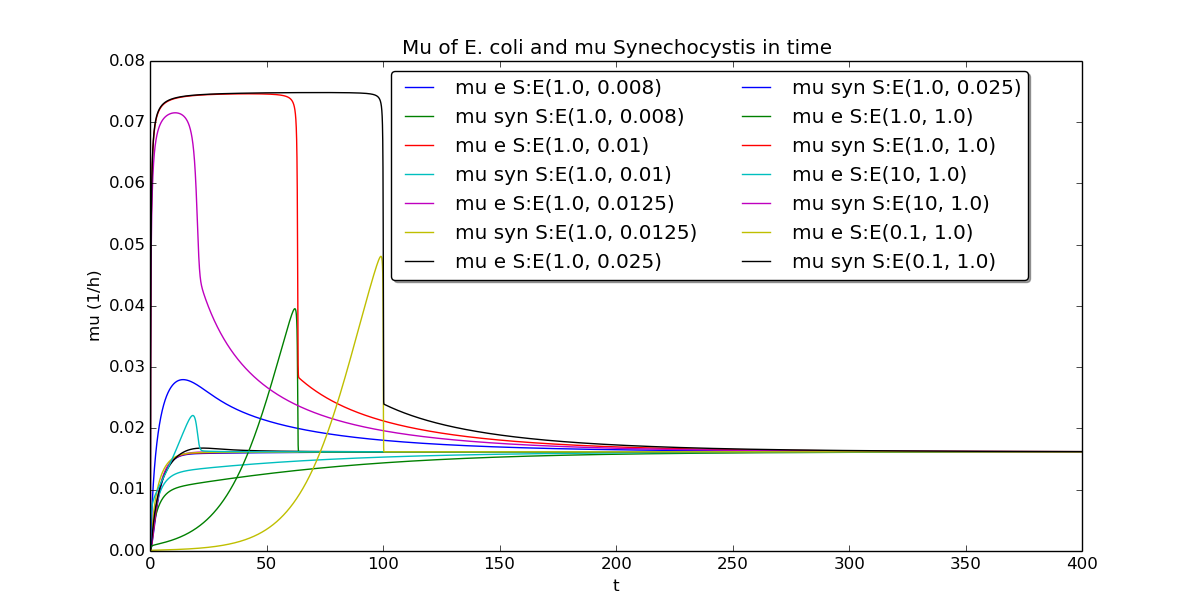
\includegraphics[width=10cm]{ratios_interdependence_mus.png}
     \caption{$\mu_{syn}$ and $\mu_{ec}$ under several different initial conditions (shown in legend in $gDW\cdot \text{l}^{-1}$). The $\mu_{ec}$ and $\mu_{syn}$ converge both to the same value. The model is given by equations \ref{eq:sd}. Parameters are given by table \ref{tab:sdp}.}
    \label{fig:submu}
    \end{center}
\end{figure}

\begin{figure}[!ht]
 \begin{center}  
     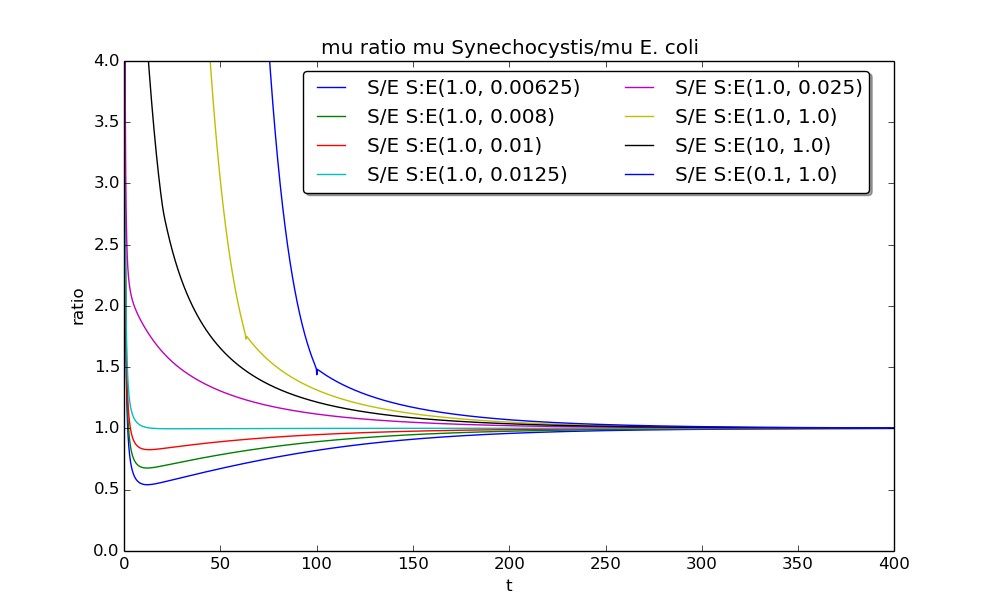
\includegraphics[width=10cm]{ratios_interdependent_muratio.png}
     \caption{Ratio between $\mu_{syn}$ and $\mu_{ec}$ under several different initial conditions (shown in legend in $gDW\cdot \text{l}^{-1}$). The $\mu_{ec}$ and $\mu_{syn}$ both converge to the same value, so the ratio converges to one. The model is given by equations \ref{eq:sd}. Parameters are given by table \ref{tab:sdp}.}
    \label{fig:submurat}
    \end{center}
\end{figure}

\pagebreak
\newpage

\subsection{Turbidostat}
In a turbidostat you can assume the growth won't be light limited, since every time a threshold OD is measured, the culture is diluted. This means you can regulate the light intensity in such a way, it won't become limiting.\\
This is why we chose to mainly look at the consequences of growing a consortium with a substrate dependent photoautotroph in a turbidostat. So the model we use is described in equations \ref{eq:turb} to \ref{eq:turbend} in section \ref{sec:turb}. The parameters used are given in table \ref{tab:sdp}
In a turbidostat it is expected that the total amount of biomass, so that if \textit{E. coli} and \textit{Synechocystis} combined would stay constant. To test this, we have plotted the total amount of biomass under different initial conditions. The result is show in figure \ref{fig:subturbtb}, and we can see that this is indeed constant. \\
This however, does not mean that the amount of biomass of each species stays the same. In figure \ref{fig:subturbbex} several examples of the amount of biomass in time of \textit{Synechocystis} and \textit{E. coli} are given.

\begin{figure}[htbp]
  \hfill
  \begin{minipage}[t]{.45\textwidth}
 \begin{center}  
     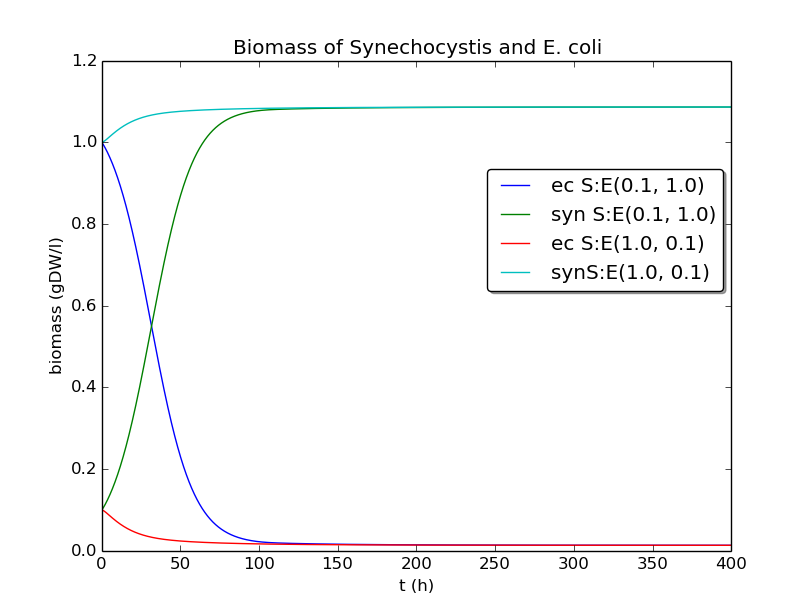
\includegraphics[width=8cm]{sub_dependent_turb_biomassex.png}
     \caption{Biomass of \textit{Synechocystis} and \textit{E. coli} in time in a turbidostat. Even thought the total amount stays the same, the amount of each species varies in time.}
    \label{fig:subturbbex}
    \end{center}
  \end{minipage}
  \hfill
  \begin{minipage}[t]{.45\textwidth}
    \begin{center}  
     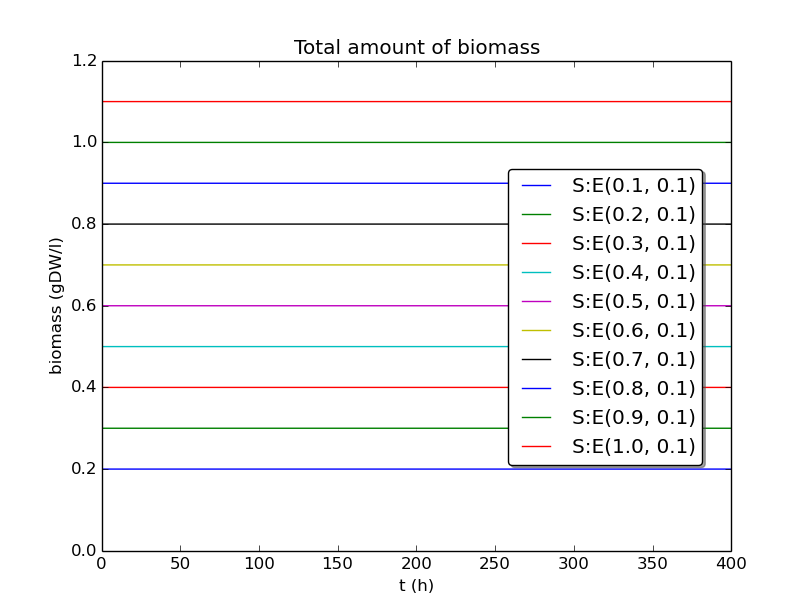
\includegraphics[width=8cm]{total_biomass1.png}
     \caption{The added biomass of \textit{Synechocystis} and \textit{E. coli} in a turbidostat. Like expected this amount stays constant.}
    \label{fig:subturbtb}
    \end{center}
  \end{minipage}
  \hfill
\end{figure}

% \begin{figure}[!ht]
%  \begin{center}  
%      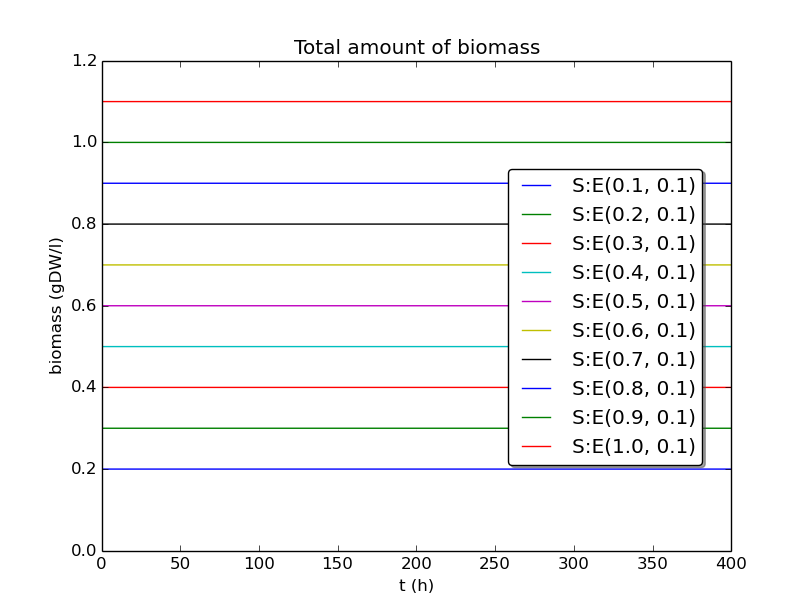
\includegraphics[width=10cm]{total_biomass1.png}
%      \caption{The added biomass of \textit{Synechocystis} and \textit{E. coli} in a turbidostat. Like expected this amount stays constant.}
%     \label{fig:subturbtb}
%     \end{center}
% \end{figure}

% \begin{figure}[!ht]
%  \begin{center}  
%      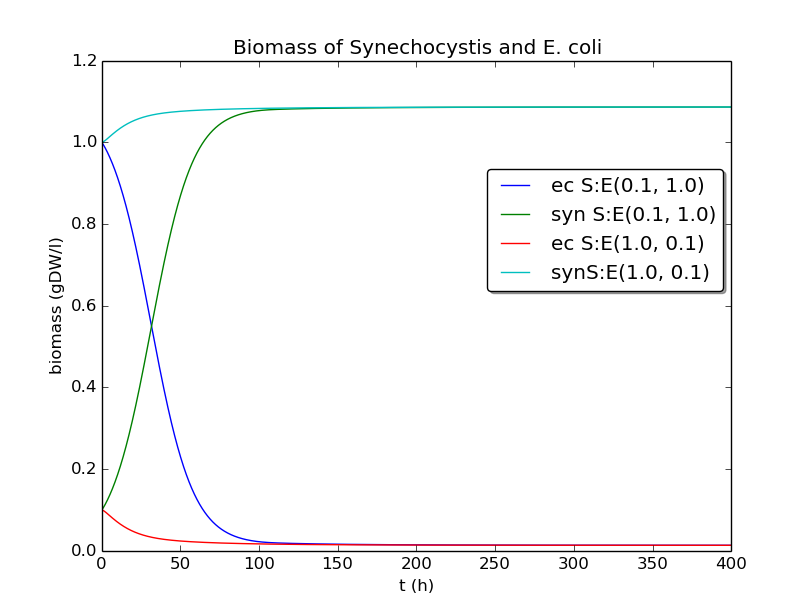
\includegraphics[width=10cm]{sub_dependent_turb_biomassex.png}
%      \caption{Biomass of \textit{Synechocystis} and \textit{E. coli} in time in a turbidostat. Even thought the total amount stays the same, the amount of each species varies in time.}
%     \label{fig:subturbbex}
%     \end{center}
% \end{figure}

Now we can once again look at the biomass ratio to see if this converges. In figure \ref{fig:subratturb} the biomass ratio in time is given under different initial conditions.

\begin{figure}[!ht]
 \begin{center}  
     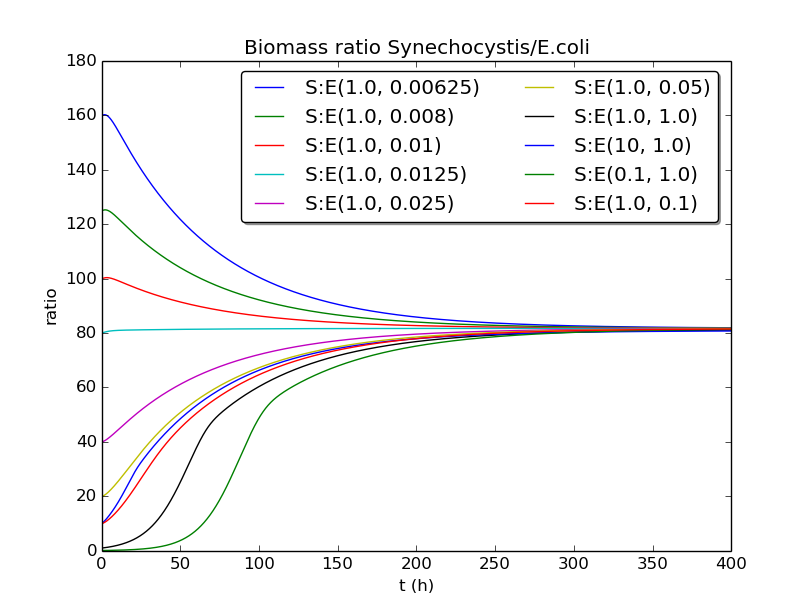
\includegraphics[width=10cm]{sub_dependent_turbidostat_bratio.png}
     \caption{Ratio of the biomass of \textit{Synechocystis} and \textit{E. coli} under several different initial conditions (shown in legend in $gDW\cdot \text{l}^{-1}$) in a turbidostat. The biomass ratio of \textit{Synechocystis} and \textit{E. coli} converge to the same value for each initial condition. The model is given by equations \ref{eq:sd}. Parameters are given by table \ref{tab:sdp}.}
    \label{fig:subratturb}
    \end{center}
\end{figure}

We can see that indeed the biomass ratio converges. Also if we look at the values for $\mu$ in figure \ref{fig:submusratturb} in time and the ratio of $mu$ in time in figure \ref{fig:submratturb}, we can see that the growth rates converge. In a turbidostat the dilution rate will become equal to this final growth rate. We can conclude that this system is also robust with respect to the initial conditions.

\begin{figure}[!ht]
 \begin{center}  
     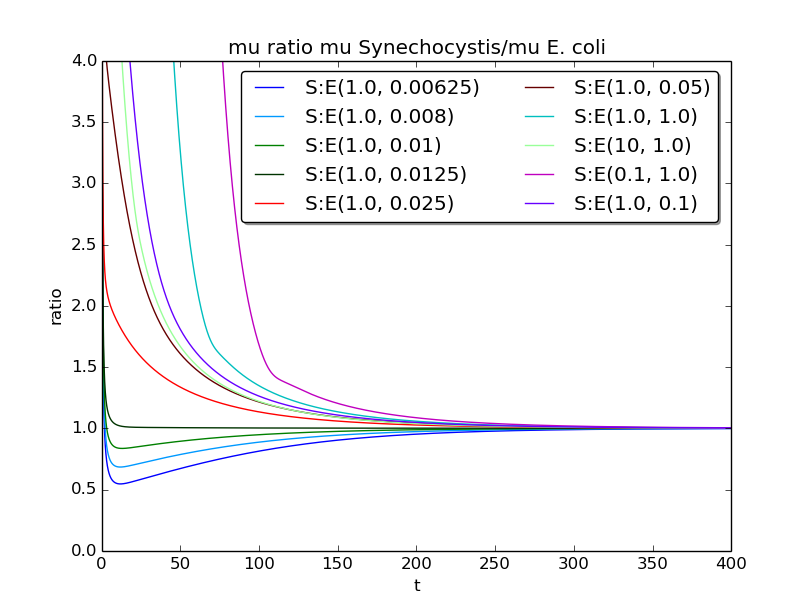
\includegraphics[width=10cm]{sub_dependent_turbidostat_muratio.png}
     \caption{Ratio of $\mu_{syn}$ and $\mu_{ec}$ under several different initial conditions (shown in legend in $gDW\cdot \text{l}^{-1}$) in a turbidostat. $\mu_{ec}$ and $\mu_{syn}$ both converge to the same value, so the ratio converges to one. The model is given by equations \ref{eq:sd}. Parameters are given by table \ref{tab:sdp}.}
    \label{fig:submratturb}
    \end{center}
\end{figure}

\begin{figure}[!ht] 
 \begin{center}  
     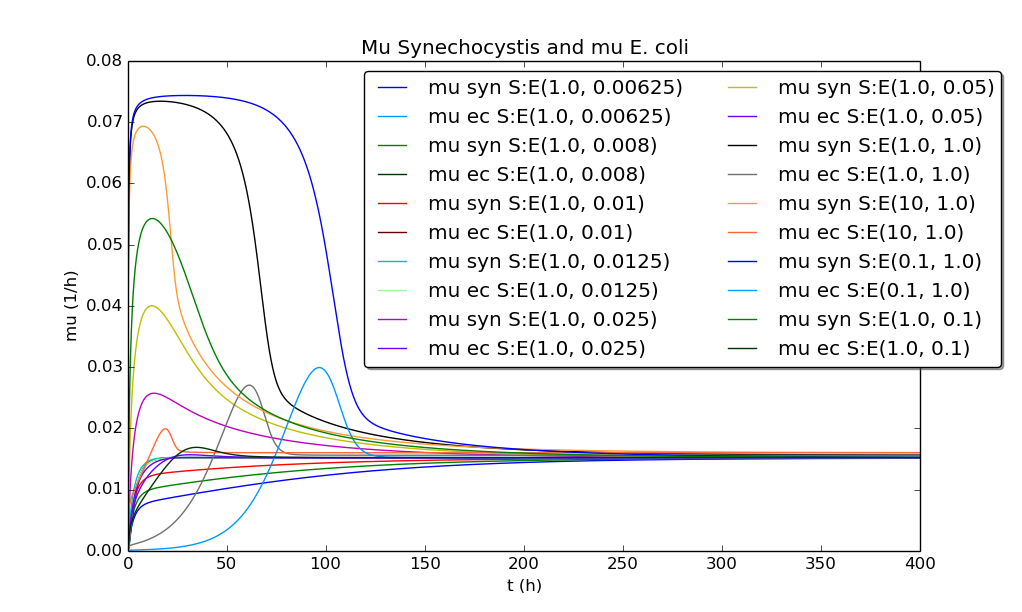
\includegraphics[width=10cm]{sub_dependent_turbidostat_mus.png}
     \caption{$\mu_{ec}$ and $\mu_{syn}$ in time in a turbidostat. $\mu_{ec}$ and $\mu_{syn}$ both converge to the same value, this value is equal to the dilution rate $D$. The model is given by equations \ref{eq:sd}. Parameters are given by table \ref{tab:sdp}.}
    \label{fig:submusratturb}
    \end{center}
\end{figure}

% \begin{figure}[!ht]
%  \begin{center}  
%      \includegraphics[width=10cm]{}
%      \caption{Limited growth on a substrate according to the Monod equation. $\mu$ is the normalized growth rate in units per hour $\mu_{max}$ is the maximal growth rate and $[S]$ is the substrate concentration. $k_S$ is the concentration at the rate equal to 
%      $\frac{1}{2} \mu_{max}$.}
%     \label{}
%     \end{center}
% \end{figure}



The models for substrate dependencies are based on the Monod equation. We created models for a consortium with a single dependency of \textit{E. coli} on a substrate \textit{Synechocystis} produces, for a consortium with a substrate interdependency, in which \textit{Synechocystis} is also dependent on a substrate \textit{E. coli} produces, and for a consortium in which \textit{Synechocystis} is growing light limited. For each of these consortia we created a model for a turbidostat environment and for batch cultures. In this handout we will show you the model we created for a substrate interdependent consortium in a turbidostat environment and we will show you the results.
\section{Turbidostat model for a substrate interdependent consortium}\label{sec:turb}
If we want to model the consortium in a turbidostat, we have to account for the fact that both \textit{Synechocystis} and E. coli are increasing the OD as they grow. This means that the dilution rate is dependent on the biomass of \textit{Synechocystis} as well as that of E. coli.
For simplicity we make the assumption that there is a constant flow through the system, instead of only diluting when the threshold is reached.  To understand this we first look at the case of a single strain, called $b$. In a chemostat the growth rate of the organism would become equal to the dilution rate. In a turbidostat however, an organism can grow at its maximal growth rate, but the amount of biomass must still become constant. This means the following:
\begin{equation}
 \frac{db}{dt} = \mu \cdot b - D \cdot b = 0
\end{equation}
Where $b$ is the amount of biomass of the strain $b$, mu is the growth rate and $D$ the dilution rate.\\
In a chemostat it would mean that $D<\mu_{max}$ is a chosen dilution rate and that $\mu$ becomes equal to $D$ due to substrate limitation. In a turbidostat however, $D$ becomes equal to $\mu_{max}$, because the species in not growing limited.\\
In the case where there are two strains, strain $a$ and $b$, that share a turbidostat, the differential equations that then describe the system looks like the following:
\begin{align}
 \frac{da}{dt} &= f(a,b,t) - Da\\
 \frac{db}{dt} &= g(a,b,t) - Db
\end{align}
Herein are $f$ and $g$ functions that describe the growth of the organisms $a$ and $b$ respectively. $D$ is again the dilution rate. Now in a shared turbidostat it holds that $a+b=k$, where $k$ is a constant amount of biomass. This implies: 
\begin{equation}
 D = \frac{g + f}{a+b}
\end{equation}

% \begin{alignat}{3}
%  & a+b &= k \\
%  &\implies \frac{da}{dt} + \frac{db}{dt} &= 0\\
%  &\implies f - Da + g - Db & = 0\\
%  &\implies Da + Db &= g + f \\
%  &\implies D &= \frac{g + f}{a+b}
% \end{alignat}
For the turbidostat we then arrive at the following set of differential equations:
\begin{align} \label{eq:turb}
 \frac{d\text{syn}}{dt} &= \mu_{syn}\cdot\text{syn} - D\cdot\text{syn}\\
 \frac{d\text{ec}}{dt} &= \mu_{ec}\cdot\text{ec} - D\cdot\text{ec} \\
 \frac{d[S_1]}{dt} &= \frac{1}{y_{syn/S1}}\cdot \mu_{syn}\cdot \text{syn} - \frac{1}{y_{ec/S1}}\cdot \mu_{ec}\cdot \text{ec} -D\cdot[S_1]\\
 \frac{d[S_2]}{dt} &=  Qp_{S2/ec}\cdot\text{ec} - \frac{1}{y_{syn/S2}}\cdot \mu_{syn}\cdot \text{syn} -D\cdot[S_2]
\end{align}
where
\begin{align}
 D &= \frac{\mu_{syn} + \mu_{ec}}{\text{syn}+\text{ec}}\\
 \mu_{syn} &= \mu_{max,syn} \frac{[S_2]}{k_{s2,syn}+[S_{2}]}\\
 \mu_{ec} &= \mu_{max,ec} \frac{S_1}{k_{s1,ec}+[S_1]} \label{eq:turbend}
\end{align}
Herein is syn the amount of biomass of \textit{Synechocystis} and ec the amount of biomass of \textit{E. coli}. 
The $\mu$s are growth rates.
$\mu_{max}$ is the maximal growth rate (equal to the growth rate at unlimited growth), and $[S]$ the concentration of substrate. $k_S$ is the concentration of $[S]$ at a rate $\frac{1}{2}\mu_{max}$. In this case there are two $\mu$ and two $\mu_{max}$ values, one for \textit{Synechocystis} and one for \textit{E. coli}. There are also two substrates. $[S_1]$ can be seen as acetate. It is being produced by \textit{Synechocystis} and consumed by \textit{E. coli}. Its production is growth coupled. $S_2$ could be arginine, It is produced by \textit{E. coli}, not in a growth coupled way, and consumed by \textit{Synechocystis}.
$y_{syn/S1}$ is the substrate yield of \textit{Synechocystis}. Since in this model the substrate is only formed when \textit{Synechocystis} forms biomass, per amount of biomass formed, there is a constant amount of substrate formed. The yield is usually expressed in gram dry weight mole substrate \emph{used}. In this case we mean gram dry weight mole substrate \emph{formed}. So to find the amount of substrate that is formed per amount of biomass that is formed we simply take $\frac{1}{y_{syn/S1}}$. $y_{ec/S1}$ and $y_{syn/S2}$ are biomass yields.

\subsection{Parameters}
To simulate the interdependency on substrates, we needed a lot more parameters. For some of the parameters we had no good measurements, so we estimated them. The general behavior stays generally the same under variations in parameters, although exact outcomes may differ.

\begin{table}[!ht]
 \begin{center}  
  \begin{tabular}{|l|l|}
   \hline
   $\mu_{max,syn}$ ($\text{h}^{-1}$) & 0.075 \\ \hline
   $\mu_{max,ec}$ ($\text{h}^{-1}$) & 0.08 \\ \hline
   $k_{s1,ec}$ ($\text{mM}$) & 0.02 \\ \hline
   $k_{s2,syn}$ ($\text{mM}$) & 0.02 \\ \hline
   $y_{\frac{s1}{syn}}$ ($\text{mmol}\cdot\text{gDW}^{-1}$) & 0.40 \\ \hline
   $y_{\frac{ec}{s}}$ ($\text{gDW}\cdot\text{mmol}^{-1}$) & 0.031 \\ \hline
   $y_{\frac{s2}{syn}}$ ($\text{mmol}\cdot\text{gDW}^{-1}$) & 0.1 \\ \hline
   $Q_{p,ec} mmol$ ($\text{mmol}\cdot \text{gDW}^{-1}\cdot\text{h}^{-1}$) & 0.13 \\
   \hline   
  \end{tabular}
  \caption{Measured and estimated parameters for the substrate interdependent model.}
  \label{tab:sdp}
 \end{center}
\end{table}

\section{Results}
% \subsection{Batch}
% \subsubsection{One-way dependency}
% First we simulated the one-way dependent model as depicted by equations \ref{eq:ow}. 
% To find out whether the system is robust with respect to the initial conditions we did some simulations. Our expectations were that the biomass ratio of the photoautotroph and the chemoheterotroph in this model would converge irrespective to the initial conditions.
% To find out whether the biomass ratio of this system converges, we did some simulations. To be able to make simulations with the models, we have to estimate and measure the parameters.
% We tried to measure all parameters as accurate as possible. In table \ref{tab:ol} the measured parameters are given.
% 
% 
% \begin{table}[!ht]
%  \begin{center}  
%   \begin{tabular}{|l|l|}
%    \hline
%    $\mu_{max,syn}$ ($\text{h}^{-1}$) & 0.075 \\ \hline
%    $\mu_{max,ec}$ ($\text{h}^{-1}$) & 0.08 \\ \hline
%    $k_{s,ec}$ ($\text{mM}$) & 0.02 \\ \hline
%    $y_{\frac{s}{syn}}$ ($\text{mmol}\cdot\text{gDW}^{-1}$) & 0.40 \\ \hline
%    $y_{\frac{ec}{s}}$ ($\text{gDW}\cdot\text{mmol}^{-1}$) & 0.031 \\
%    \hline   
%   \end{tabular}
%   \caption{Measured parameters for the one-way dependency model. It can be seen that $\mu_{max,ec} < \mu_{max,syn}$. This is highly unlikely the correct value for $\mu{max,ec}$}
%   \label{tab:ol}
%  \end{center}
% \end{table}
% 
% It can be seen from this table, that $\mu_{max,ec} < \mu_{max,syn}$. It is very unlikely that this is correct. It might be caused by experimental Since $\mu$ of \textit{Synechocystis} higher than the $\mu_{max}$ of \textit{E. coli} and given that the growth of \textit{Synechocystis} is independent, we can already expect this model with these parameter to be unstable. \textit{Synechocystis} will keep growing faster than \textit{E. coli}, because the growth rate of \textit{Synechocystis} has a constant value that is higher than the maximal growth rate \textit{E. coli} will ever achieve. If we simulate the model with these parameters find the biomass ratio given in figure \ref{fig:false}. It can be seen that the ratio of biomass does not seem to converge. A more clear image can be seen if we look at the $mu$'s of \textit{E. coli} and \textit{Synechocystis} in figure \ref{fig:false2}.
% 
% \begin{figure}[!ht]
%  \begin{center}  
%      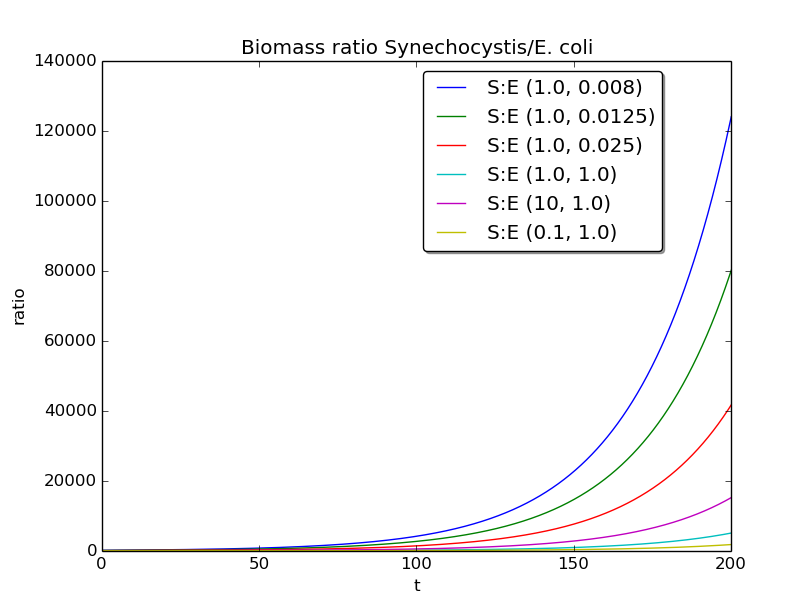
\includegraphics[width=10cm]{independent_flask_ratios_low_mumaxe.png}
%      \caption{Boiomass ratio's of \textit{Synechocystis}/\textit{E. coli} in time. They seem to diverge, dependent on the initial conditions. This seems logical, since the growth rate of \textit{E. coli} will never become as high as that of \textit{Synechocystis}. In the legend the initial ratio of \textit{Synechocystis} biomass : \textit{E. coli} biomass is given. The model is given by equations \ref{eq:ow}. Parameters are given by table \ref{tab:ol}}
%     \label{fig:false}
%     \end{center}
% \end{figure}
% 
% 
% \begin{figure}[!ht]
%  \begin{center}  
%      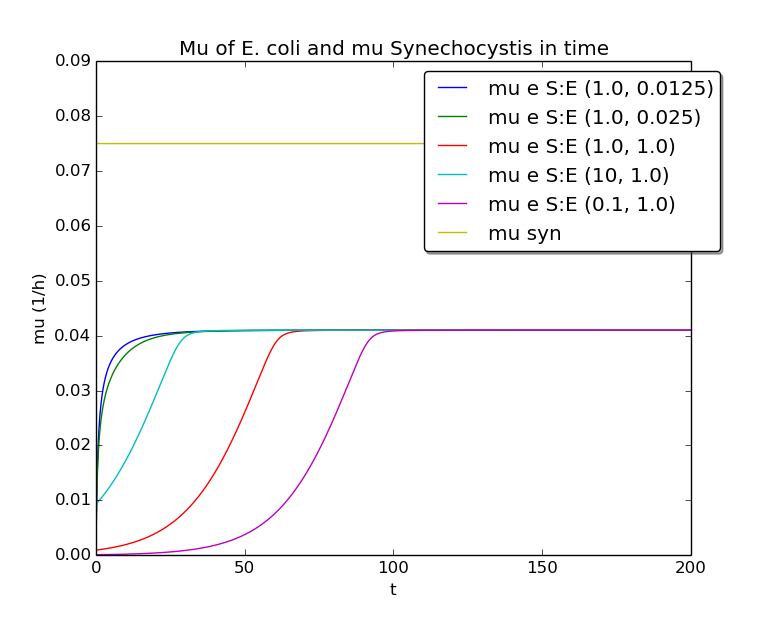
\includegraphics[width=10cm]{independent_flask_mus_low_mumaxe.png}
%      \caption{$\mu_{syn}$ and $\mu_{ec}$ under several different initial conditions (shown in legend in $gDW\cdot \text{l}^{-1}$). $\mu_{ec}$ converges to $\mu_{max,ec}$, while $\mu_{syn}$ stays constant at the value of $\mu_{max,syn}$. The model is given by equations \ref{eq:ow}. Parameters are given by table \ref{tab:ol}}
%     \label{fig:false2}
%     \end{center}
% \end{figure}
% 
% Chemoheterotrophs are usually have a really high growth rate compared to photoautotrophs. Even though the maximal growth rate of \textit{E. coli} on Acetate might be less than the maximal growth rate on glucose, it is very unlikely that the maximal growth rate is less than that of Synechocystis. So, the question remains, will the biomass ratio converge if we change the parameters such that $\mu_{max,ec} > \mu_{max,syn}$?
% To test this we have increased $\mu_{max,ec}$ tot 0.08, which is just higher than the growth rate of Synechocystis. In table \ref{tab:oh} the new parameters are shown.
% 
% \begin{table}[!ht]
%  \begin{center}  
%   \begin{tabular}{|l|l|}
%    \hline
%    $\mu_{max,syn}$ ($\text{h}^{-1}$) & 0.075 \\ \hline
%    $\mu_{max,ec}$ ($\text{h}^{-1}$) & 0.08 \\ \hline
%    $k_{s,ec}$ ($\text{mM}$) & 0.02 \\ \hline
%    $y_{\frac{s}{syn}}$ ($\text{mmol}\cdot\text{gDW}^{-1}$) & 0.40 \\ \hline
%    $y_{\frac{ec}{s}}$ ($\text{gDW}\cdot\text{mmol}^{-1}$) & 0.031 \\
%    \hline   
%   \end{tabular}
%   \caption{Measured and estimated parameters for the one-way dependency model. It can be seen that now $\mu_{max,ec} > \mu_{max,syn}$.}
%   \label{tab:oh}
%  \end{center}
% \end{table}
% 
% In figure \ref{fig:oneratio}, the biomass ratio over time given several different initial conditions is shown. Now the biomass ratio does seem to converge. However, this ratio is more than ten times higher than what is found in the lab. This might suggest that we still use inaccurately measured parameters. 
% 
% \begin{figure}[!ht]
%  \begin{center}  
%      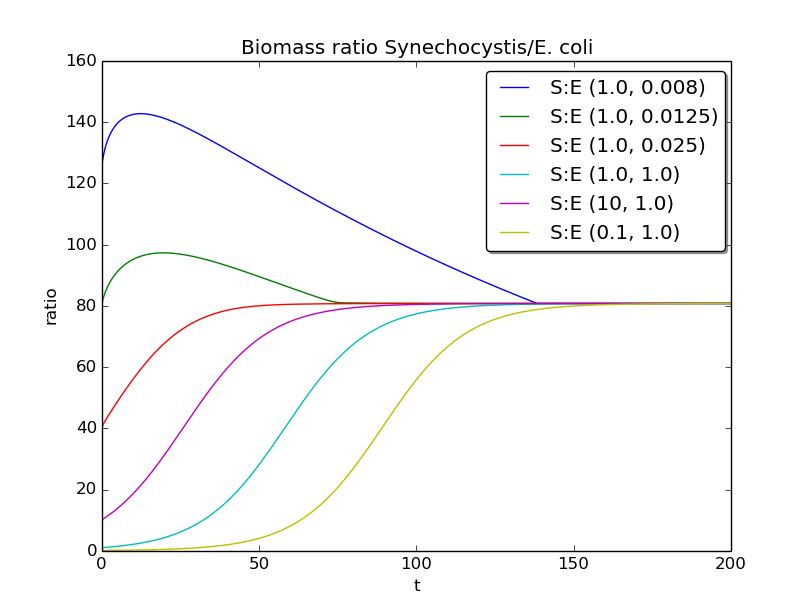
\includegraphics[width=10cm]{independent_flask_ratios.png}
%      \caption{The biomass ratio of \textit{Synechocystis} \textit{E. coli} under several different initial conditions (shown in legend in $gDW\cdot \text{l}^{-1}$). The biomass ratio converges to a constant ratio. The model is given by equations \ref{eq:ow}. Parameters are given by table \ref{tab:oh}}
%     \label{fig:oneratio}
%     \end{center}
% \end{figure}
% 
% If we look once again at the $\mu$'s over time in figure \ref{fig:onemu} we can see that the $\mu_{ec}$ converges to $\mu_{sys}$. This is quite intuitive, since the growth rate of \textit{E. coli} is limited by the production of substrate, which is dependent on the growth rate of \textit{Synechocystis}. And the biomasses can only converge to a stable ratio, if the growth rates of both species converge to the same value. 
% We can conclude that the system now is robust with respect to the initial values.
% 
% \begin{figure}[!ht]
%  \begin{center}  
%      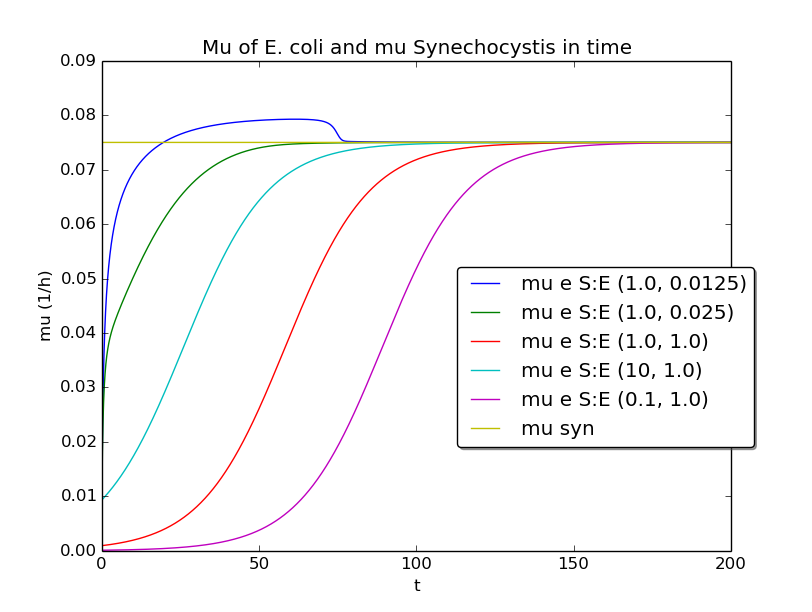
\includegraphics[width=10cm]{independent_flask_mus.png}
%      \caption{$\mu_{syn}$ and $\mu_{ec}$ under several different initial conditions (shown in legend in $gDW\cdot \text{l}^{-1}$). The $\mu_{ec}$ converges to $\mu_{syn}=\mu_{max,syn}$. The model is given by equations \ref{eq:ow}. Parameters are given by table \ref{tab:oh}.}
%     \label{fig:onemu}
%     \end{center}
% \end{figure}

% \subsection{Parameters}
% To simulate the interdependency on substrates, we needed a lot more parameters. For some of the parameters we had no good measurements, so we estimated them. The general behavior stays generally the same under variations in parameters, although exact outcomes may differ.
% 
% \begin{table}[!ht]
%  \begin{center}  
%   \begin{tabular}{|l|l|}
%    \hline
%    $\mu_{max,syn}$ ($\text{h}^{-1}$) & 0.075 \\ \hline
%    $\mu_{max,ec}$ ($\text{h}^{-1}$) & 0.08 \\ \hline
%    $k_{s1,ec}$ ($\text{mM}$) & 0.02 \\ \hline
%    $k_{s2,syn}$ ($\text{mM}$) & 0.02 \\ \hline
%    $y_{\frac{s1}{syn}}$ ($\text{mmol}\cdot\text{gDW}^{-1}$) & 0.40 \\ \hline
%    $y_{\frac{ec}{s}}$ ($\text{gDW}\cdot\text{mmol}^{-1}$) & 0.031 \\ \hline
%    $y_{\frac{s2}{syn}}$ ($\text{mmol}\cdot\text{gDW}^{-1}$) & 0.1 \\ \hline
%    $Q_{p,ec} mmol$ ($\text{mmol}\cdot \text{gDW}^{-1}\cdot\text{h}^{-1}$) & 0.13 \\
%    \hline   
%   \end{tabular}
%   \caption{Measured and estimated parameters for the substrate interdependent model.}
%   \label{tab:sdp}
%  \end{center}
% \end{table}
% 
% 
% \begin{figure}[!ht]
%  \begin{center}  
%      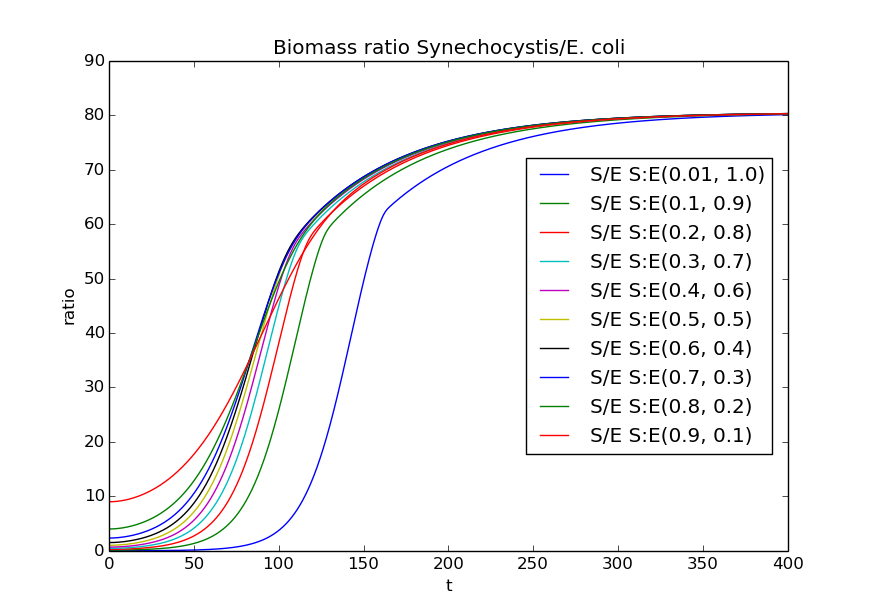
\includegraphics[width=10cm]{ratios_interdependent_1.png}
%      \caption{The biomass ratio of \textit{Synechocystis} \textit{E. coli} under several different initial conditions (shown in legend in $gDW\cdot \text{l}^{-1}$). The biomass ratio converges to a constant ratio. The model is given by equations \ref{eq:sd}. Parameters are given by table \ref{tab:sdp}}
%     \label{fig:subrat}
%     \end{center}
% \end{figure}
% 
% \begin{figure}[!ht]
%  \begin{center}  
%      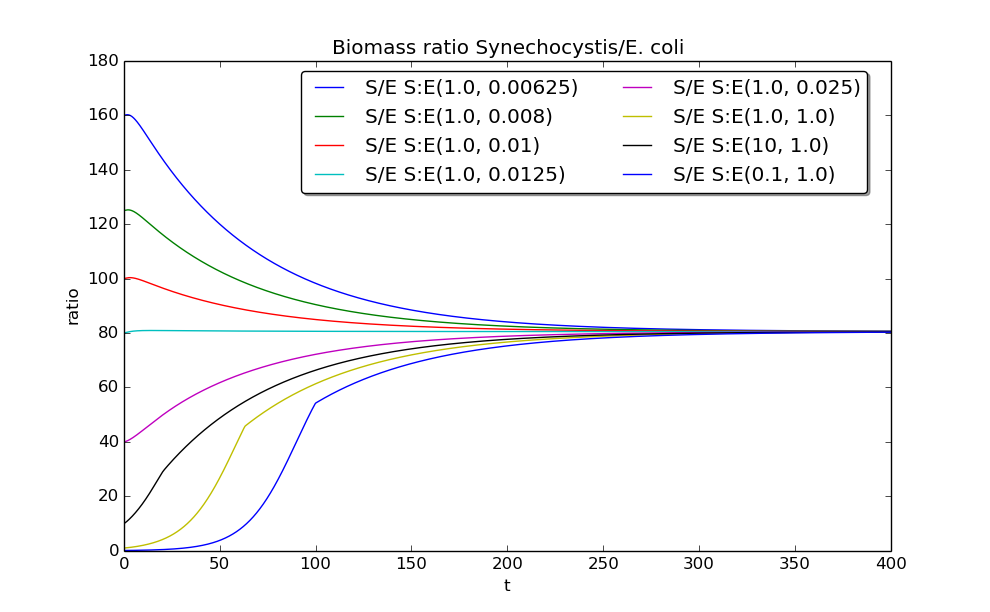
\includegraphics[width=10cm]{ratios_interdependent_2.png}
%      \caption{The biomass ratio of \textit{Synechocystis} \textit{E. coli} under several different initial conditions (shown in legend in $gDW\cdot \text{l}^{-1}$). The biomass ratio converges to a constant ratio. The model is given by equations \ref{eq:sd}. Parameters are given by table \ref{tab:sdp}}
%     \label{fig:subrat2}
%     \end{center}
% \end{figure}
% 
% 
% \begin{figure}[!ht]
%  \begin{center}  
%      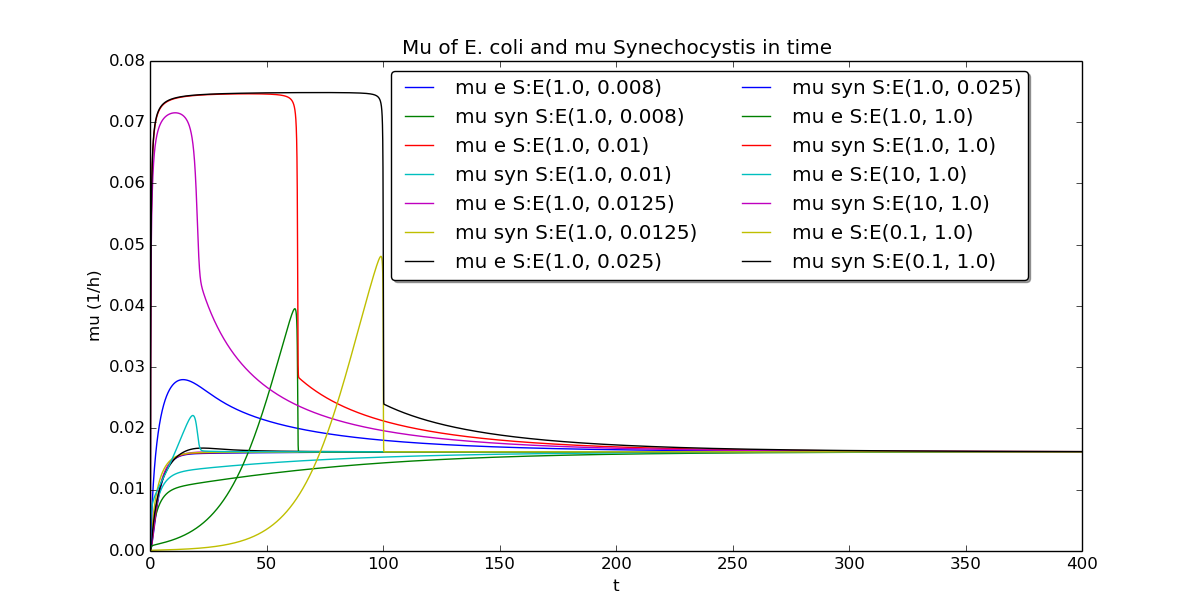
\includegraphics[width=10cm]{ratios_interdependence_mus.png}
%      \caption{$\mu_{syn}$ and $\mu_{ec}$ under several different initial conditions (shown in legend in $gDW\cdot \text{l}^{-1}$). The $\mu_{ec}$ and $\mu_{syn}$ converge both to the same value. The model is given by equations \ref{eq:sd}. Parameters are given by table \ref{tab:sdp}.}
%     \label{fig:submu}
%     \end{center}
% \end{figure}
% 
% \begin{figure}[!ht]
%  \begin{center}  
%      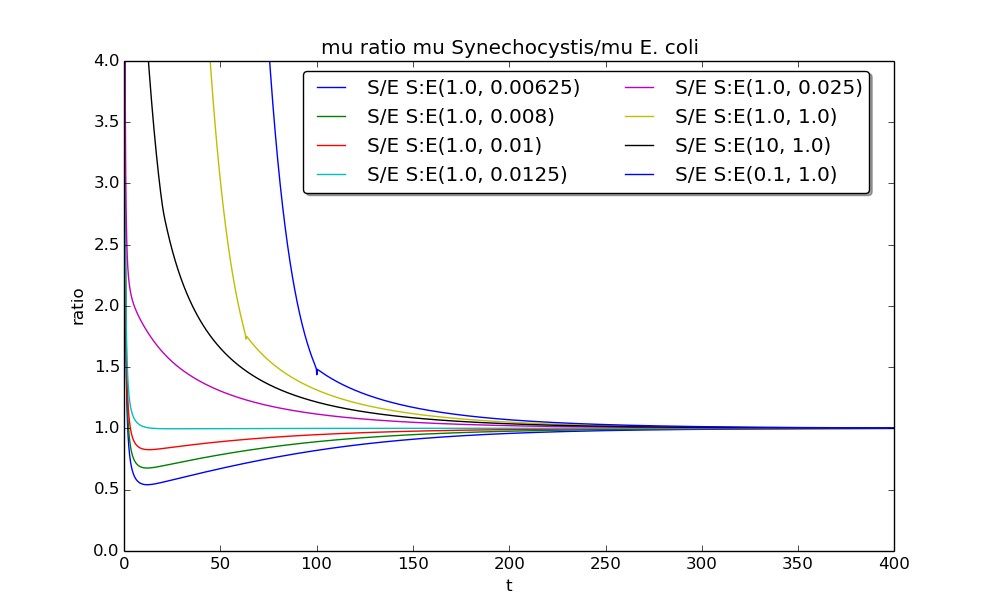
\includegraphics[width=10cm]{ratios_interdependent_muratio.png}
%      \caption{Ratio between $\mu_{syn}$ and $\mu_{ec}$ under several different initial conditions (shown in legend in $gDW\cdot \text{l}^{-1}$). The $\mu_{ec}$ and $\mu_{syn}$ both converge to the same value, so the ratio converges to one. The model is given by equations \ref{eq:sd}. Parameters are given by table \ref{tab:sdp}.}
%     \label{fig:submurat}
%     \end{center}
% \end{figure}
% 
% \pagebreak
% \newpage

Here we will show you some results of the simulations of a consortium with a substrate dependent photoautotroph in a turbidostat. The model we used is described in equations \ref{eq:turb} to \ref{eq:turbend} in section \ref{sec:turb}. The parameters used are given in table \ref{tab:sdp}
In a turbidostat it is expected that the total amount of biomass, so that if \textit{E. coli} and \textit{Synechocystis} combined would stay constant. To test this, we have plotted the total amount of biomass under different initial conditions. The result is show in figure \ref{fig:subturbtb}, and we can see that this is indeed constant. \\
This however, does not mean that the amount of biomass of each species stays the same. In figure \ref{fig:subturbbex} several examples of the amount of biomass in time of \textit{Synechocystis} and \textit{E. coli} are given.

\begin{figure}[htbp]
  \hfill
  \begin{minipage}[t]{.45\textwidth}
 \begin{center}  
     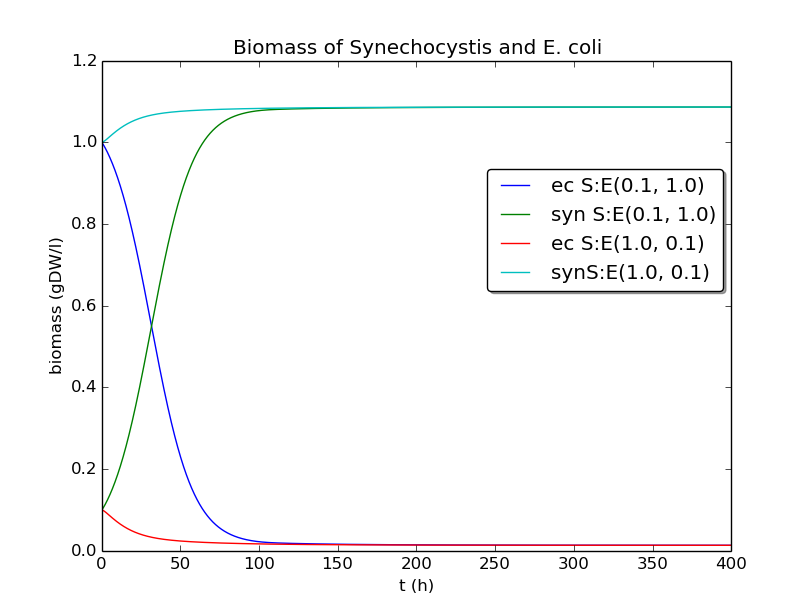
\includegraphics[width=7.5cm]{sub_dependent_turb_biomassex.png}
     \caption{Biomass of \textit{Synechocystis} and \textit{E. coli} in time in a turbidostat. Even thought the total amount stays the same, the amount of each species varies in time.}
    \label{fig:subturbbex}
    \end{center}
  \end{minipage}
  \hfill
  \begin{minipage}[t]{.45\textwidth}
    \begin{center}  
     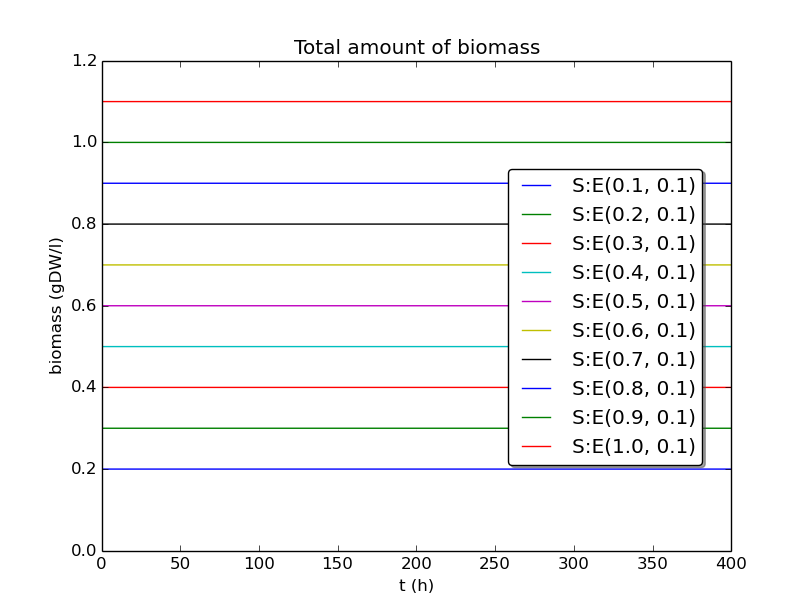
\includegraphics[width=7.5cm]{total_biomass1.png}
     \caption{The added biomass of \textit{Synechocystis} and \textit{E. coli} in a turbidostat. Like expected this amount stays constant.}
    \label{fig:subturbtb}
    \end{center}
  \end{minipage}
  \hfill
  \begin{minipage}{.45\textwidth}
   \begin{center}
         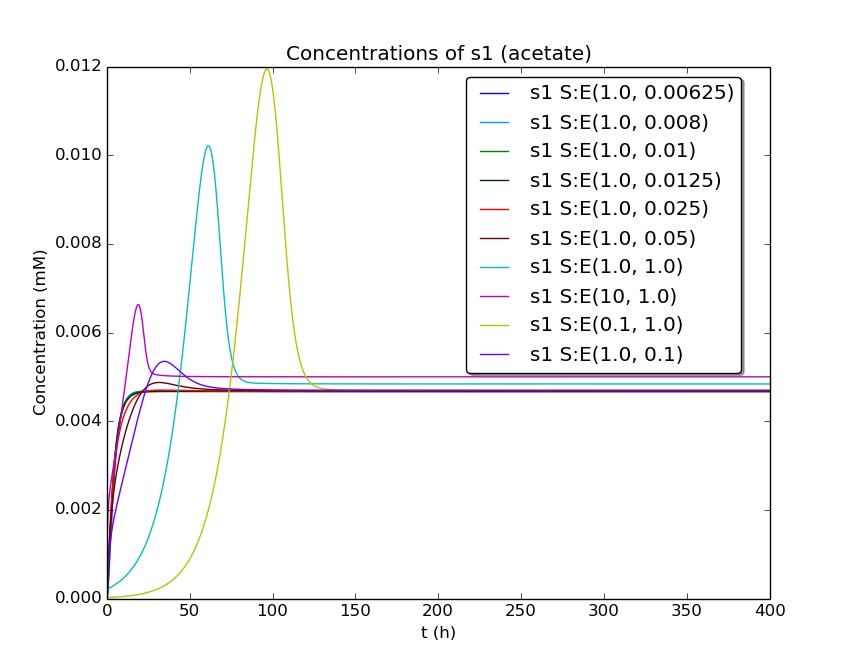
\includegraphics[width=7.5cm]{S1.png}
     \caption{Concentration of acetate, or $S_1$ in the model in time under different initial conditions. After an initial spike it stabelizes.}
    \label{fig:s1}
   \end{center}
  \end{minipage}
    \hfill
  \begin{minipage}{.45\textwidth}
   \begin{center}
         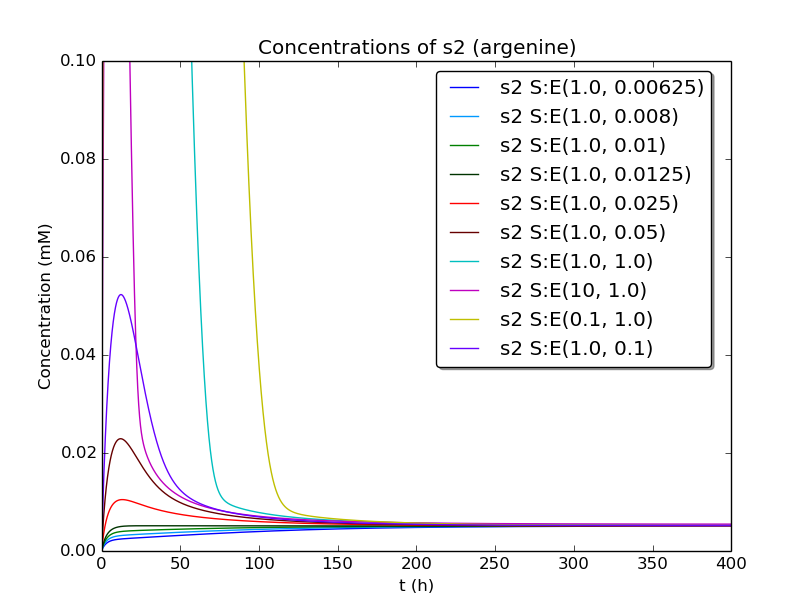
\includegraphics[width=7.5cm]{S2.png}
     \caption{Concentration of argenine, or $S_2$ in the model in time under different initial conditions. After an initial spike it stabelizes}
    \label{fig:s2}
   \end{center}
  \end{minipage}
    \hfill
  \begin{minipage}{.45\textwidth}
   \begin{center}
     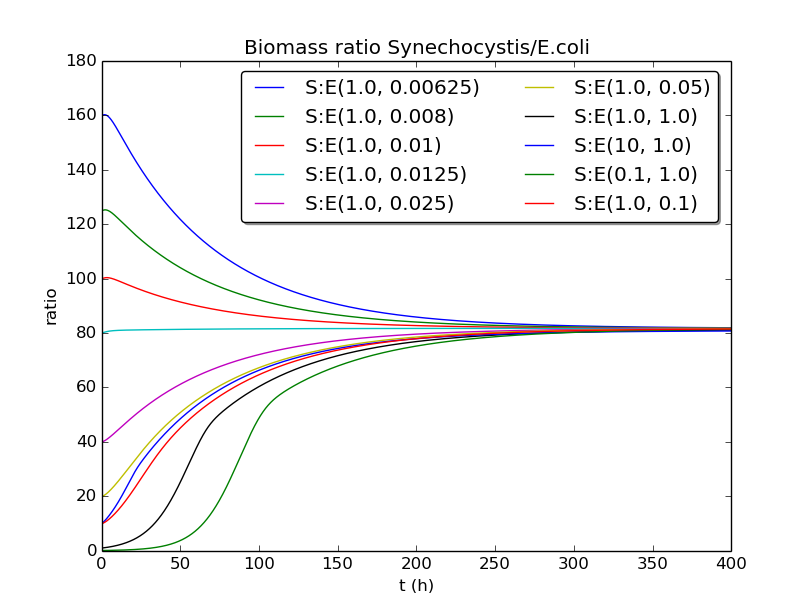
\includegraphics[width=7.5cm]{sub_dependent_turbidostat_bratio.png}
     \caption{Ratio of the biomass of \textit{Synechocystis} and \textit{E. coli} under several different initial conditions (shown in legend in $gDW\cdot \text{l}^{-1}$) in a turbidostat. The biomass ratio of \textit{Synechocystis} and \textit{E. coli} converge to the same value for each initial condition. The model is given by equations \ref{eq:turb} to \ref{eq:turbend}. Parameters are given by table \ref{tab:sdp}.}
     \label{fig:subratturb}
   \end{center}
  \end{minipage}
    \hfill
  \begin{minipage}{.45\textwidth}
   \begin{center}
     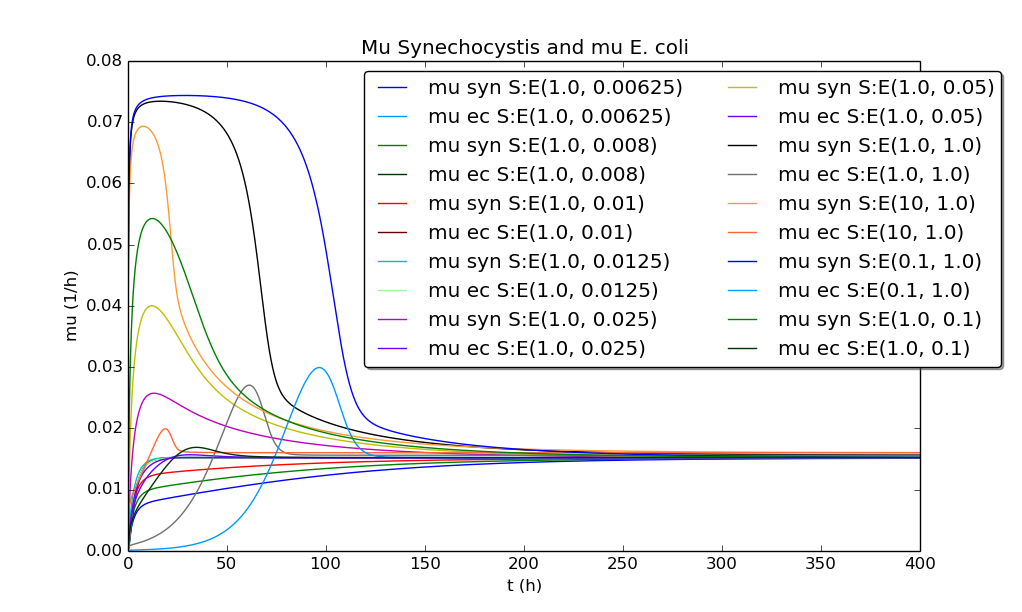
\includegraphics[width=7.5cm]{sub_dependent_turbidostat_mus.png}
     \caption{$\mu_{ec}$ and $\mu_{syn}$ in time in a turbidostat. $\mu_{ec}$ and $\mu_{syn}$ both converge to the same value, this value is equal to the dilution rate $D$. The model is given by equations \ref{eq:turb} to \ref{eq:turbend}. Parameters are given by table \ref{tab:sdp}.}
    \label{fig:submusratturb}
   \end{center}
  \end{minipage}
\end{figure}

% \begin{figure}[!ht]
%  \begin{center}  
%      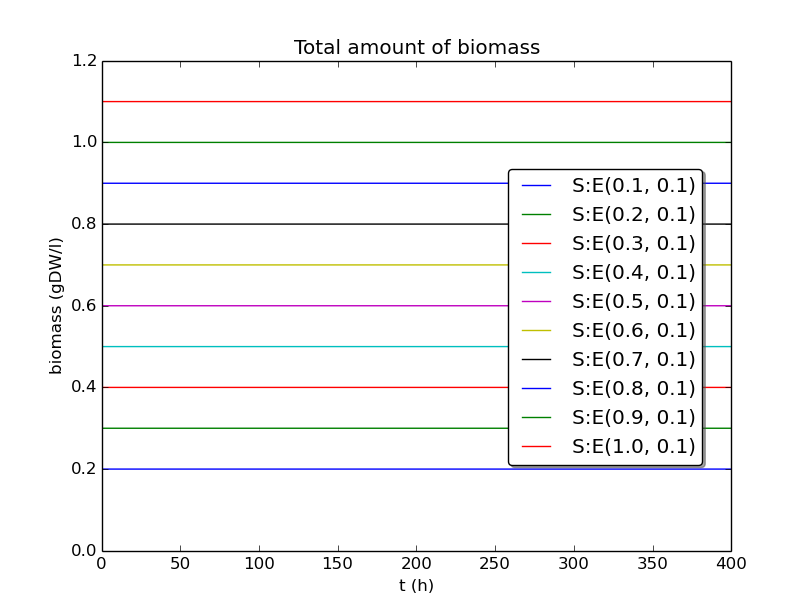
\includegraphics[width=10cm]{total_biomass1.png}
%      \caption{The added biomass of \textit{Synechocystis} and \textit{E. coli} in a turbidostat. Like expected this amount stays constant.}
%     \label{fig:subturbtb}
%     \end{center}
% \end{figure}

% \begin{figure}[!ht]
%  \begin{center}  
%      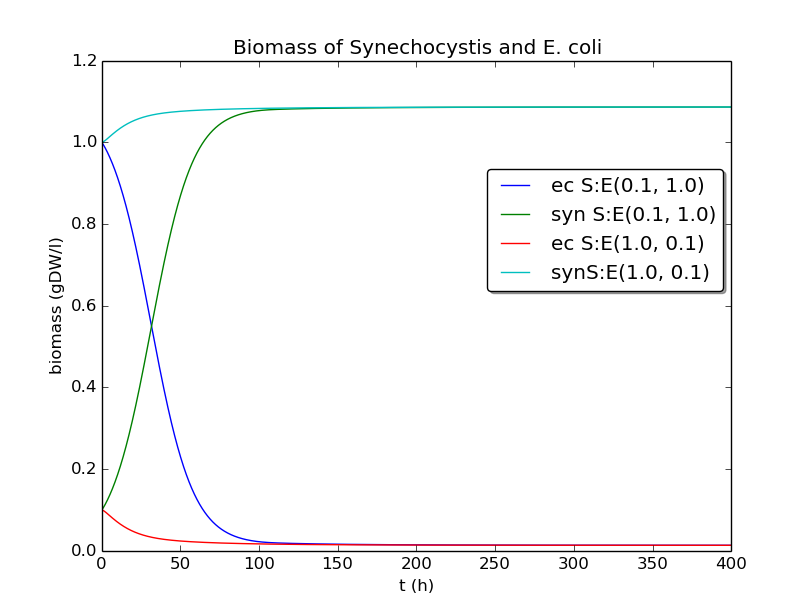
\includegraphics[width=10cm]{sub_dependent_turb_biomassex.png}
%      \caption{Biomass of \textit{Synechocystis} and \textit{E. coli} in time in a turbidostat. Even thought the total amount stays the same, the amount of each species varies in time.}
%     \label{fig:subturbbex}
%     \end{center}
% \end{figure}

Now we can once again look at the biomass ratio to see if this converges. In figure \ref{fig:subratturb} the biomass ratio in time is given under different initial conditions.

% \begin{figure}[!ht]
%  \begin{center}  
%      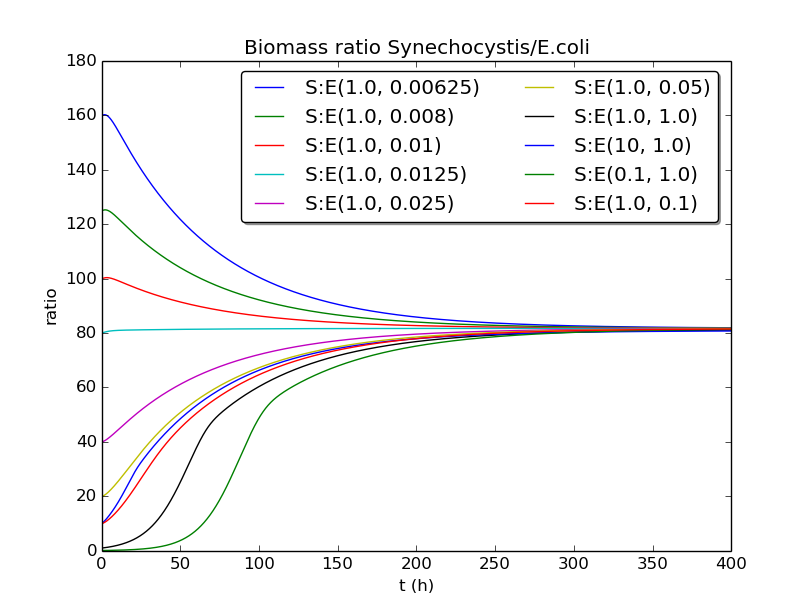
\includegraphics[width=10cm]{sub_dependent_turbidostat_bratio.png}
%      \caption{Ratio of the biomass of \textit{Synechocystis} and \textit{E. coli} under several different initial conditions (shown in legend in $gDW\cdot \text{l}^{-1}$) in a turbidostat. The biomass ratio of \textit{Synechocystis} and \textit{E. coli} converge to the same value for each initial condition. The model is given by equations \ref{eq:sd}. Parameters are given by table \ref{tab:sdp}.}
%     \label{fig:subratturb}
%     \end{center}
% \end{figure}

We can see that indeed the biomass ratio converges. Also if we look at the values for $\mu$ in figure \ref{fig:submusratturb} in time, we can see that the growth rates converge. In a turbidostat the dilution rate will become equal to the final growth rate to which the growth rates converge. We can also conclude that this system stabilizes in time and that it is robust with respect to the initial conditions. 

% \begin{figure}[!ht]
%  \begin{center}  
%      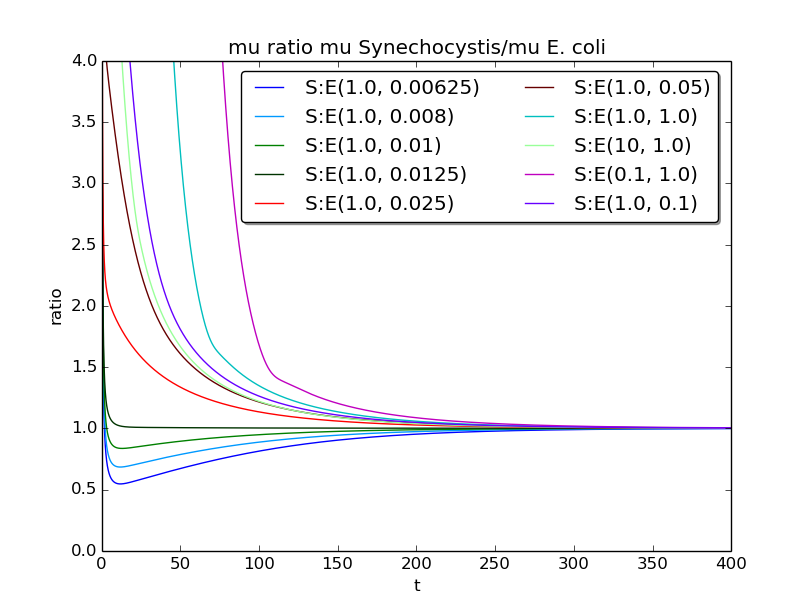
\includegraphics[width=10cm]{sub_dependent_turbidostat_muratio.png}
%      \caption{Ratio of $\mu_{syn}$ and $\mu_{ec}$ under several different initial conditions (shown in legend in $gDW\cdot \text{l}^{-1}$) in a turbidostat. $\mu_{ec}$ and $\mu_{syn}$ both converge to the same value, so the ratio converges to one. The model is given by equations \ref{eq:turb} to \ref{eq:turbend}. Parameters are given by table \ref{tab:sdp}.}
%     \label{fig:submratturb}
%     \end{center}
% \end{figure}

% \begin{figure}[!ht] 
%  \begin{center}  
%      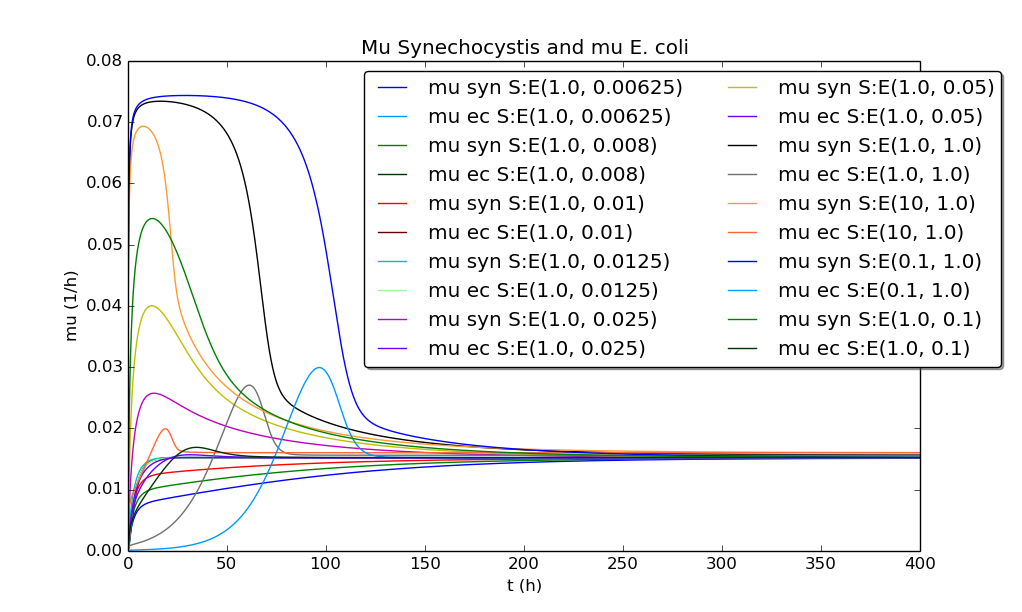
\includegraphics[width=10cm]{sub_dependent_turbidostat_mus.png}
%      \caption{$\mu_{ec}$ and $\mu_{syn}$ in time in a turbidostat. $\mu_{ec}$ and $\mu_{syn}$ both converge to the same value, this value is equal to the dilution rate $D$. The model is given by equations \ref{eq:sd}. Parameters are given by table \ref{tab:sdp}.}
%     \label{fig:submusratturb}
%     \end{center}
% \end{figure}

% \begin{figure}[!ht]
%  \begin{center}  
%      \includegraphics[width=10cm]{}
%      \caption{Limited growth on a substrate according to the Monod equation. $\mu$ is the normalized growth rate in units per hour $\mu_{max}$ is the maximal growth rate and $[S]$ is the substrate concentration. $k_S$ is the concentration at the rate equal to 
%      $\frac{1}{2} \mu_{max}$.}
%     \label{}
%     \end{center}
% \end{figure}


%\bibliographystyle{unsrtnat}
%\bibliography{iGEMrefs}



\begin{abstract}
  
\end{abstract}

\section{Introduction}
Why do we want to use kinetic models?
Under what restrictions does a symbiosis converge.
When is something considered stable?

\section{Methods}
type of models
sets of differential equations
software

\section{Results}
convergenge
pictures
toepassing (Stijn en Hugo)
stability analysis

\section{Discussion}
Different values than Stijn's values
maybe add delay to get oscillations in future research
too much combinations of parameters
too much parameters

\chapter{Discussion}
Results in the light of the iGEM project
Why a 2 organisms, why symbiose, complications with 2 organisms in a tank
How to advance.


\chapter{Acknowledgement}


\bibliographystyle{unsrtnat}
\bibliography{iGEMrefs}
\end{document}
